\chapter{Result}

\section{How to evaluate}
In this project, we need to manually count the number of contrails and evaluate the correctness of all results with different parameters. \\

\subsection{Detect Rules}
Here are the rules to count the contrails and detected lines:\\
\begin{enumerate}
    \item the contrails and result lines are counted manually
    \item in the origin image and final output image, we only count the lines with clear boarder
    \item if two lines are overlay each other, and the angle between two lines are less than 5 degree, we count it as one
    \item if the lines are more than 10 and hard to count the number, we count it as 10, because the default maximum number of lines to detect is 10 in the Hough Transform in MatLab.
\end{enumerate}

\subsection{Parameters Definition}
Here are the definitions of parameters used in my program:
\begin{itemize}
    \item Block Radius is the size of blocks in the process of reduce bad pixels. According to our algorithm, for each pixel, we need to do check all the pixels around it within the block radius to check if there is/are line(s) across this block.\\
    \item Percentage is the percentage of best blocks to keep in the final step of algorithm to reduce bad edgels. \\
    \item Fill Gap is a build-in parameter in the Hough Transform, if there are two line segments are in same slope but no parallel and their distance are less than Fill Gap, the Hough Transform will concatenate two line segments and consider them as one line.\\
    \item Minimum Length is a build-in parameter in the Hough Transfer, only if the line segment is larger than a certain length (MinLength), then it will be considered. \\
\end{itemize}


\section{Results and Discussion}
According to the results of program's giving, we sort it by largest correct rate firstly and least incorrect rate secondly. Then we can have some discussion here.

\clearpage
\subsection{Satellite Image}

Figure \ref{figure1} is a satellite image with about 7 contrails which are easier to be recognized and others are relatively blurrier.

\begin{figure}[htb!]
\centering
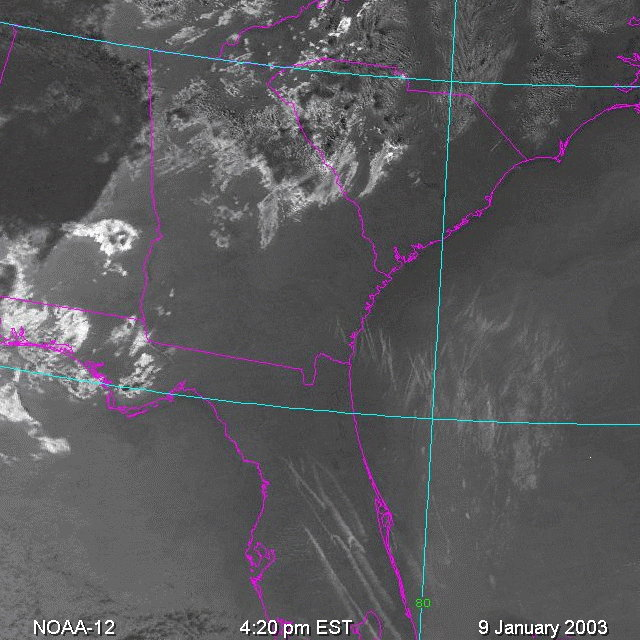
\includegraphics[width=5in]{pic/figure1.jpg}
\caption{A satellite image with longitude and latitude lines (640 x 640)}
\label{figure1}
\end{figure}

The result cannot be fully detected, with the interference of the lat-lag and broader lines.\\
The best result has the parameters with block radius as 2, percentage to keep as 15, fill gap as 600, and minimum length can be any in 25, 50 and 100. The best result of Satellite Image is greatly impacted by the lat-lag lines. It covers all the contrails, however, it also covers lots of points are not contrails. We can see the largest correct rate is even less than 50\%, which clearly shows this detective is ineffeicent. And the worst result covers a longitude line only, it doesn’t cover any contrails because that longitude line has a much more clear edge than contrails. The results image for figure \ref{figure1} can be seen at figure \ref{Figure1_best} for the best result and figure \ref{Figure1_worst} for the worst result.

\begin{figure}[hbtp]
	\centering
	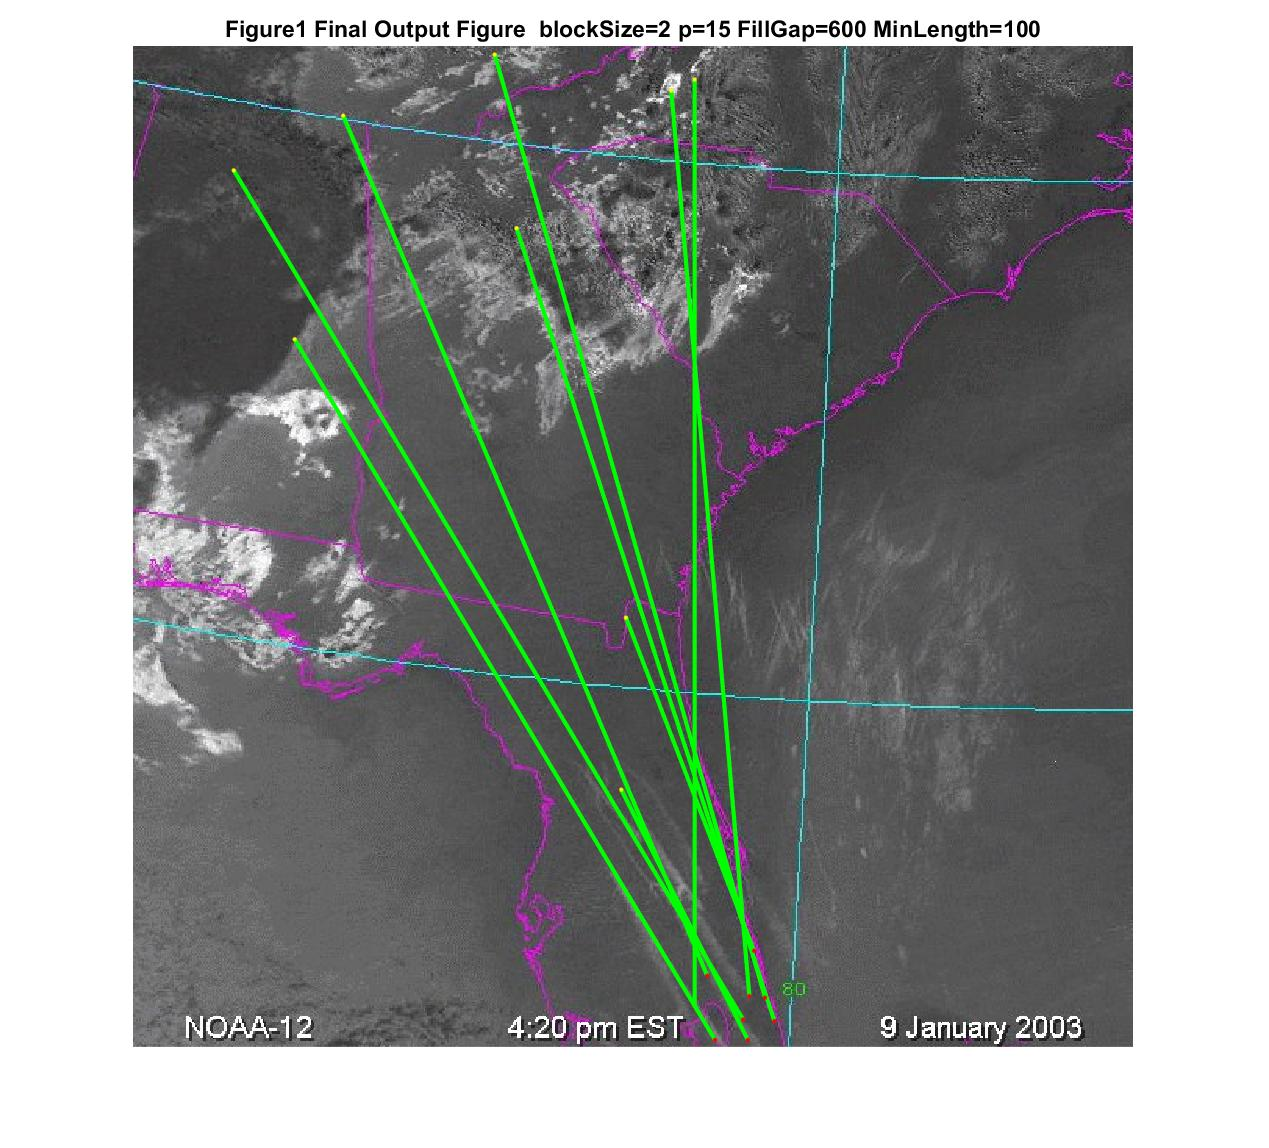
\includegraphics[width=6in]{pic/Figure1_best.jpg}
	\caption{Best Result for Figure \ref{figure1}}
	\label{Figure1_best}
\end{figure}


\begin{figure}[hbtp]
	\centering
	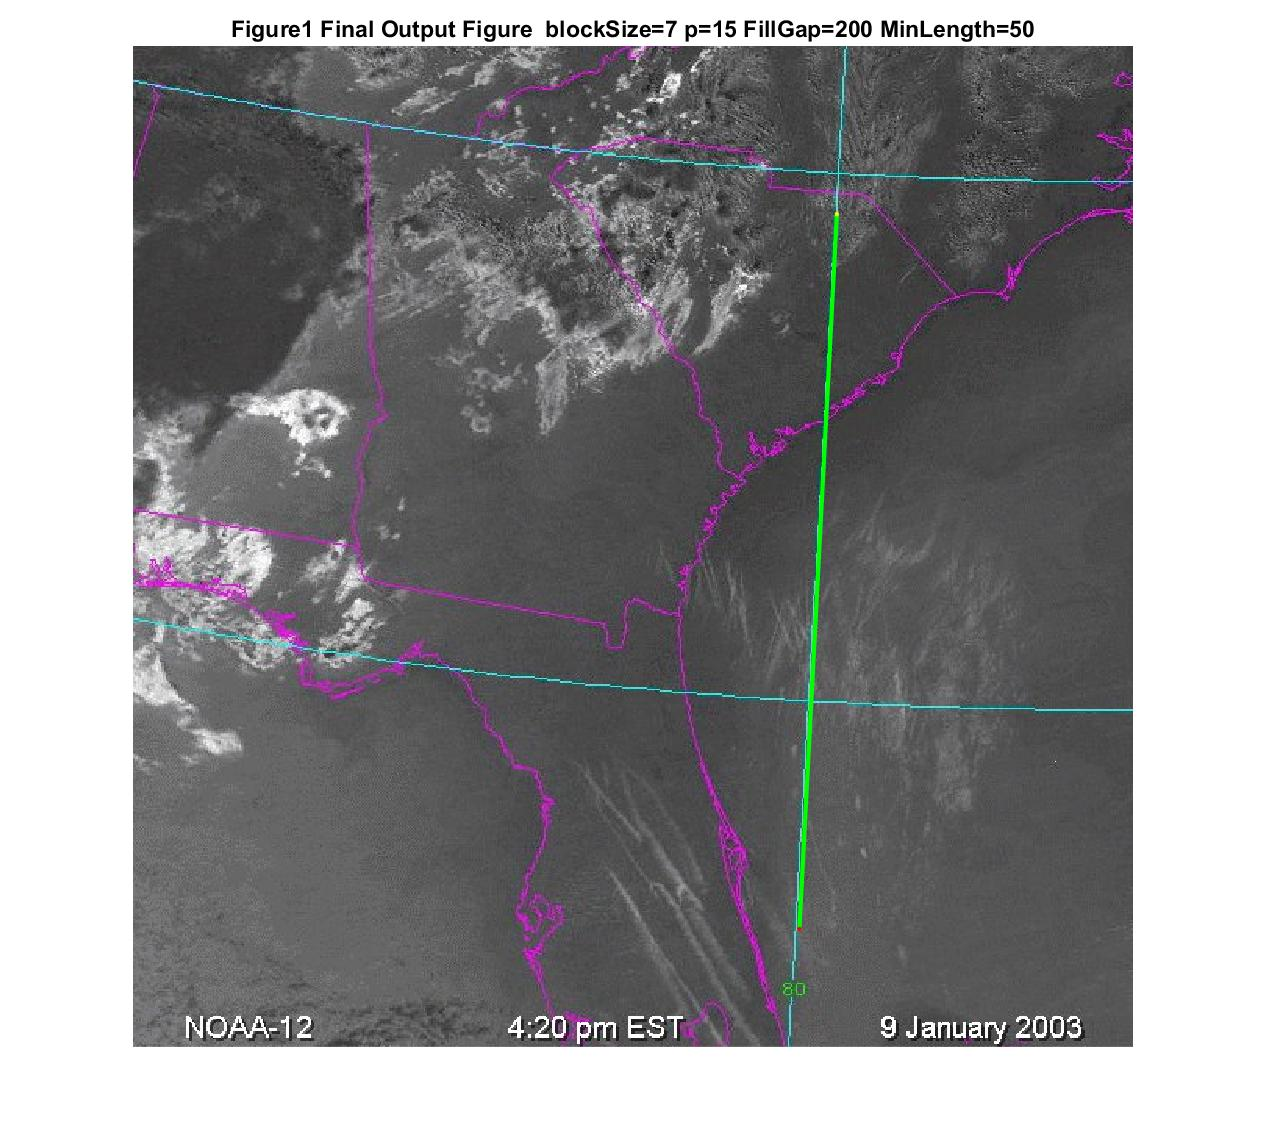
\includegraphics[width=6in]{pic/Figure1_worst.jpg}
	\caption{Worst Result for Figure \ref{figure1}, only covers lagtitude line}
	\label{Figure1_worst}
\end{figure}


\clearpage

\begingroup
\setlength{\LTleft}{-20cm plus -1fill}
\setlength{\LTright}{\LTleft}
{\small
\begin{longtable}{| c | c | c | c | c | c | c | c | c |} \hline
Block & Percentage & FillGap & Minimum & Correct & Incorrect & Missingr & Correct & Incorrect \\
Radius &  & & Length & Number & Number & Number & Rate & Rate \\ \hline
 2 & 15 & 600 & 50 & 3 & 5 & 4 & 42.86\% & 62.50\%   \\
 2 & 15 & 600 & 100 & 3 & 5 & 4 & 42.86\% & 62.50\%   \\
 2 & 15 & 600 & 25 & 3 & 5 & 4 & 42.86\% & 62.50\%   \\
 2 & 15 & 200 & 50 & 2 & 5 & 5 & 28.57\% & 71.43\%   \\
 2 & 15 & 200 & 100 & 2 & 5 & 5 & 28.57\% & 71.43\%   \\
 2 & 25 & 400 & 25 & 2 & 5 & 5 & 28.57\% & 71.43\%   \\
 2 & 25 & 400 & 50 & 2 & 5 & 5 & 28.57\% & 71.43\%   \\
 2 & 25 & 400 & 100 & 2 & 5 & 5 & 28.57\% & 71.43\%   \\
 2 & 15 & 400 & 25 & 2 & 6 & 5 & 28.57\% & 75.00\%   \\
 2 & 15 & 400 & 50 & 2 & 6 & 5 & 28.57\% & 75.00\%   \\
 2 & 15 & 400 & 100 & 2 & 6 & 5 & 28.57\% & 75.00\%   \\
 2 & 25 & 600 & 25 & 2 & 6 & 5 & 28.57\% & 75.00\%   \\
 2 & 25 & 600 & 50 & 2 & 6 & 5 & 28.57\% & 75.00\%   \\
 2 & 25 & 600 & 100 & 2 & 6 & 5 & 28.57\% & 75.00\%   \\
 2 & 15 & 200 & 25 & 2 & 7 & 5 & 28.57\% & 77.78\%   \\
 2 & 5 & 200 & 25 & 2 & 8 & 5 & 28.57\% & 80.00\%   \\
 2 & 5 & 200 & 50 & 2 & 8 & 5 & 28.57\% & 80.00\%   \\
 2 & 5 & 200 & 100 & 2 & 8 & 5 & 28.57\% & 80.00\%   \\
 2 & 5 & 400 & 25 & 2 & 9 & 5 & 28.57\% & 81.82\%   \\
 2 & 5 & 400 & 50 & 2 & 9 & 5 & 28.57\% & 81.82\%   \\
 2 & 5 & 400 & 100 & 2 & 9 & 5 & 28.57\% & 81.82\%   \\
 2 & 5 & 600 & 25 & 2 & 9 & 5 & 28.57\% & 81.82\%   \\
 2 & 5 & 600 & 50 & 2 & 9 & 5 & 28.57\% & 81.82\%   \\
 2 & 5 & 600 & 100 & 2 & 9 & 5 & 28.57\% & 81.82\%   \\
 2 & 25 & 200 & 50 & 2 & 9 & 5 & 28.57\% & 81.82\%   \\
 2 & 25 & 200 & 100 & 2 & 9 & 5 & 28.57\% & 81.82\%   \\
 2 & 25 & 200 & 25 & 2 & 10 & 5 & 28.57\% & 83.33\%   \\
 7 & 5 & 200 & 100 & 0 & 1 & 7 & 0.00\% & 100.00\%   \\
 7 & 5 & 400 & 25 & 0 & 1 & 7 & 0.00\% & 100.00\%   \\
 7 & 5 & 400 & 50 & 0 & 1 & 7 & 0.00\% & 100.00\%   \\
 7 & 5 & 400 & 100 & 0 & 1 & 7 & 0.00\% & 100.00\%   \\
 7 & 5 & 600 & 25 & 0 & 1 & 7 & 0.00\% & 100.00\%   \\
 7 & 5 & 600 & 50 & 0 & 1 & 7 & 0.00\% & 100.00\%   \\
 7 & 5 & 600 & 100 & 0 & 1 & 7 & 0.00\% & 100.00\%   \\
 7 & 15 & 200 & 25 & 0 & 1 & 7 & 0.00\% & 100.00\%   \\
 7 & 15 & 200 & 50 & 0 & 1 & 7 & 0.00\% & 100.00\%   \\
 7 & 15 & 200 & 100 & 0 & 1 & 7 & 0.00\% & 100.00\%   \\
 7 & 15 & 400 & 25 & 0 & 1 & 7 & 0.00\% & 100.00\%   \\
 7 & 15 & 400 & 50 & 0 & 1 & 7 & 0.00\% & 100.00\%   \\
  7 & 15 & 400 & 100 & 0 & 1 & 7 & 0.00\% & 100.00\%   \\
 7 & 15 & 600 & 25 & 0 & 1 & 7 & 0.00\% & 100.00\%   \\
 7 & 15 & 600 & 50 & 0 & 1 & 7 & 0.00\% & 100.00\%   \\
 7 & 15 & 600 & 100 & 0 & 1 & 7 & 0.00\% & 100.00\%   \\
 7 & 25 & 200 & 25 & 0 & 1 & 7 & 0.00\% & 100.00\%   \\
 7 & 25 & 200 & 50 & 0 & 1 & 7 & 0.00\% & 100.00\%   \\
 7 & 25 & 200 & 100 & 0 & 1 & 7 & 0.00\% & 100.00\%   \\
 7 & 25 & 400 & 25 & 0 & 1 & 7 & 0.00\% & 100.00\%   \\
 7 & 25 & 400 & 50 & 0 & 1 & 7 & 0.00\% & 100.00\%   \\
 7 & 25 & 400 & 100 & 0 & 1 & 7 & 0.00\% & 100.00\%   \\
 7 & 25 & 600 & 25 & 0 & 1 & 7 & 0.00\% & 100.00\%   \\
 7 & 25 & 600 & 50 & 0 & 1 & 7 & 0.00\% & 100.00\%   \\
 7 & 25 & 600 & 100 & 0 & 1 & 7 & 0.00\% & 100.00\%   \\
 12 & 5 & 200 & 25 & 0 & 1 & 7 & 0.00\% & 100.00\%   \\
 12 & 5 & 200 & 50 & 0 & 1 & 7 & 0.00\% & 100.00\%   \\
 12 & 5 & 200 & 100 & 0 & 1 & 7 & 0.00\% & 100.00\%   \\
 12 & 5 & 400 & 25 & 0 & 1 & 7 & 0.00\% & 100.00\%   \\
 12 & 5 & 400 & 50 & 0 & 1 & 7 & 0.00\% & 100.00\%   \\
 12 & 5 & 400 & 100 & 0 & 1 & 7 & 0.00\% & 100.00\%   \\
 12 & 5 & 600 & 25 & 0 & 1 & 7 & 0.00\% & 100.00\%   \\
 12 & 5 & 600 & 50 & 0 & 1 & 7 & 0.00\% & 100.00\%   \\
 12 & 5 & 600 & 100 & 0 & 1 & 7 & 0.00\% & 100.00\%   \\
 12 & 15 & 200 & 25 & 0 & 1 & 7 & 0.00\% & 100.00\%   \\
 12 & 15 & 200 & 50 & 0 & 1 & 7 & 0.00\% & 100.00\%   \\
 12 & 15 & 200 & 100 & 0 & 1 & 7 & 0.00\% & 100.00\%   \\
 12 & 15 & 400 & 25 & 0 & 1 & 7 & 0.00\% & 100.00\%   \\
 12 & 15 & 400 & 50 & 0 & 1 & 7 & 0.00\% & 100.00\%   \\
 12 & 15 & 400 & 100 & 0 & 1 & 7 & 0.00\% & 100.00\%   \\
 12 & 15 & 600 & 25 & 0 & 1 & 7 & 0.00\% & 100.00\%   \\
 12 & 15 & 600 & 50 & 0 & 1 & 7 & 0.00\% & 100.00\%   \\
 12 & 15 & 600 & 100 & 0 & 1 & 7 & 0.00\% & 100.00\%   \\
 12 & 25 & 200 & 25 & 0 & 1 & 7 & 0.00\% & 100.00\%   \\
 12 & 25 & 200 & 50 & 0 & 1 & 7 & 0.00\% & 100.00\%   \\
 12 & 25 & 200 & 100 & 0 & 1 & 7 & 0.00\% & 100.00\%   \\
 12 & 25 & 400 & 25 & 0 & 1 & 7 & 0.00\% & 100.00\%   \\
 12 & 25 & 400 & 50 & 0 & 1 & 7 & 0.00\% & 100.00\%   \\
 12 & 25 & 400 & 100 & 0 & 1 & 7 & 0.00\% & 100.00\%   \\
 12 & 25 & 600 & 25 & 0 & 1 & 7 & 0.00\% & 100.00\%   \\
 12 & 25 & 600 & 50 & 0 & 1 & 7 & 0.00\% & 100.00\%   \\
 12 & 25 & 600 & 100 & 0 & 1 & 7 & 0.00\% & 100.00\%   \\
 7 & 5 & 200 & 25 & 0 & 1 & 7 & 0.00\% & 100.00\%   \\
 7 & 5 & 200 & 50 & 0 & 1 & 7 & 0.00\% & 100.00\%   \\ \hline
\caption{Experimental results for Figure \ref{figure1}.}
\label{table1}
\end{longtable}
}
\endgroup

\clearpage
\subsection{Contrails in Trees and Sky Image}

Figure \ref{figure2} is a color image with 1 thin contrail which is easy to realize. However, there also exists some clear boarder of trees and sky. Even thought the boarder is clear, their edge curves are not as straight as contrails.\\
The best result happens when parameters without the block radius as 2, others can all be counted as the best, their correctness rate are 100\%, and incorrect rate are 0\%. It covers only contrail very well, only a small part of this contrail not be covered because it sightly curved. As for the worst, it happens when blockSize = 2, p = 15, FillGap = 600, MinLength = 25, it has more than 10 incorrect lines, none of them covers that contrail. The results image for figure \ref{figure2} can be seen at figure \ref{Figure2_best} for the best result and figure \ref{Figure2_worst} for the worst result.

\begin{figure}[htb!]
\centering
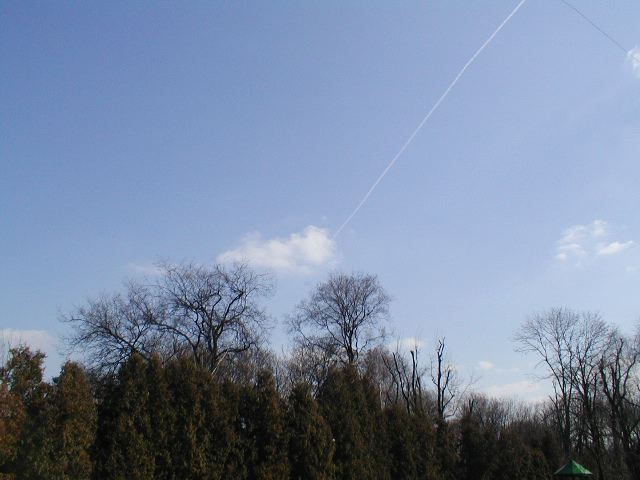
\includegraphics[width=6in]{pic/figure2.jpg}
\caption{Contrails in Trees and Sky Image (640 x 480)}
\label{figure2}
\end{figure}


\begin{figure}[hbtp]
	\centering
	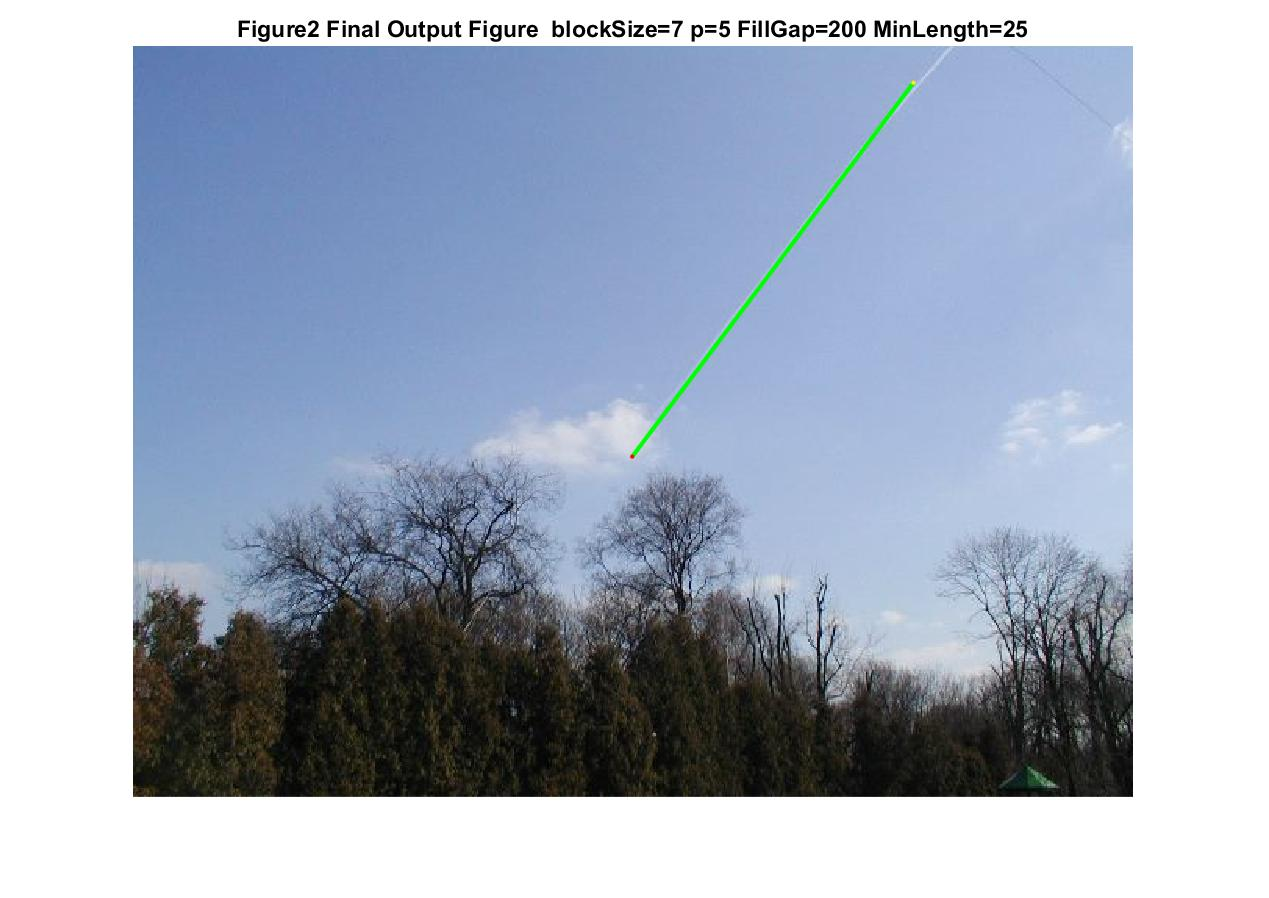
\includegraphics[width=6in]{pic/Figure2_best.jpg}
	\caption{Best Result for Figure \ref{figure2}}
	\label{Figure2_best}
\end{figure}


\begin{figure}[hbtp]
	\centering
	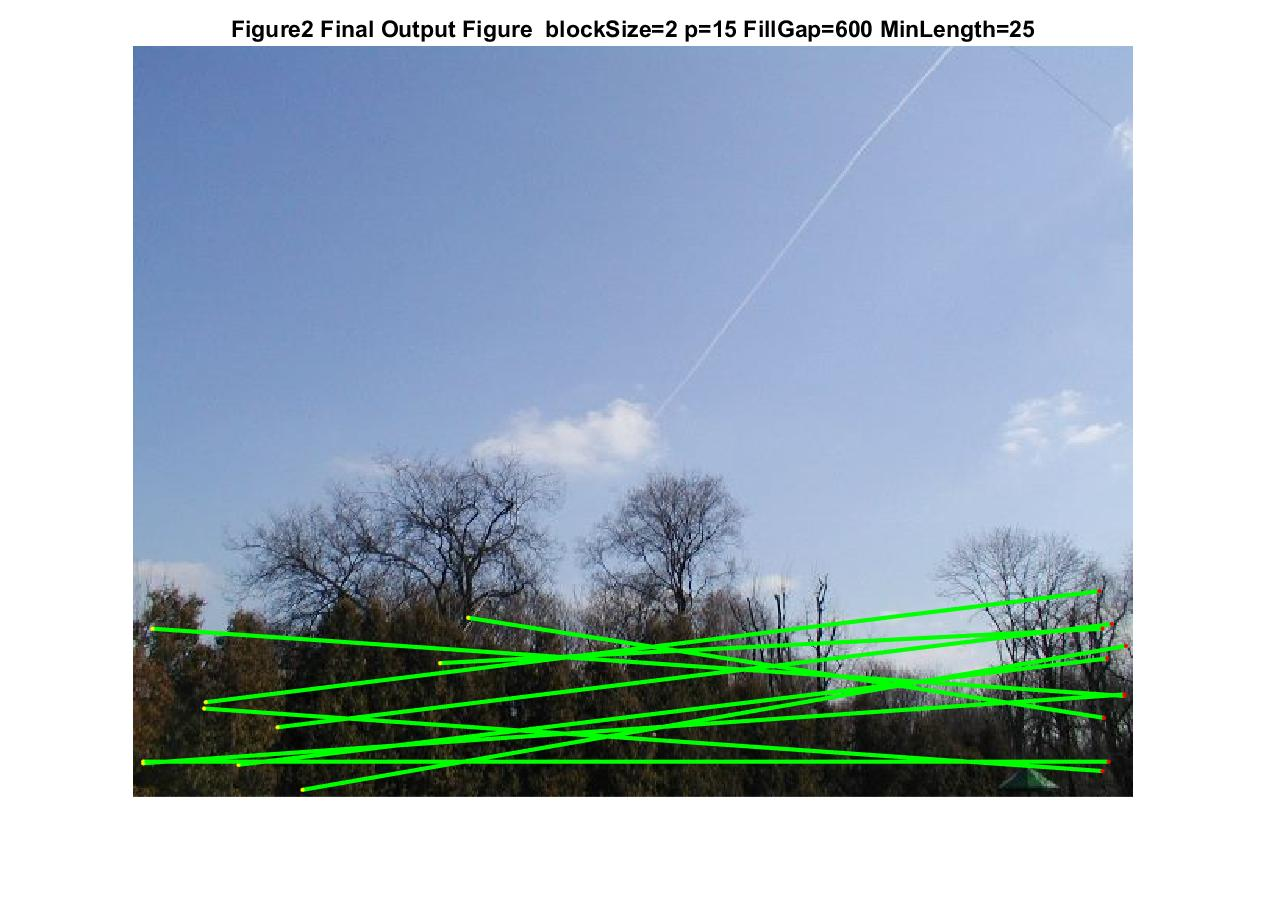
\includegraphics[width=6in]{pic/Figure2_worst.jpg}
	\caption{Worst Result for Figure \ref{figure2}, no contrail covered, and too many useless lines}
	\label{Figure2_worst}
\end{figure}


\clearpage
\begingroup
\setlength{\LTleft}{-20cm plus -1fill}
\setlength{\LTright}{\LTleft}
{\small
\begin{longtable}{| c | c | c | c | c | c | c | c | c |} \hline
Block & Percentage & FillGap & Minimum & Correct & Incorrect & Missingr & Correct & Incorrect \\
Radius &  & & Length & Number & Number & Number & Rate & Rate \\ \hline
7 & 5 & 200 & 25 & 1 & 0 & 0 & 100.00\% & 0.00\% \\
7 & 5 & 200 & 50 & 1 & 0 & 0 & 100.00\% & 0.00\% \\
7 & 5 & 200 & 100 & 1 & 0 & 0 & 100.00\% & 0.00\% \\
7 & 5 & 400 & 25 & 1 & 0 & 0 & 100.00\% & 0.00\% \\
7 & 5 & 400 & 50 & 1 & 0 & 0 & 100.00\% & 0.00\% \\
7 & 5 & 400 & 100 & 1 & 0 & 0 & 100.00\% & 0.00\% \\
7 & 5 & 600 & 25 & 1 & 0 & 0 & 100.00\% & 0.00\% \\
7 & 5 & 600 & 50 & 1 & 0 & 0 & 100.00\% & 0.00\% \\
7 & 5 & 600 & 100 & 1 & 0 & 0 & 100.00\% & 0.00\% \\
7 & 15 & 200 & 25 & 1 & 0 & 0 & 100.00\% & 0.00\% \\
7 & 15 & 200 & 50 & 1 & 0 & 0 & 100.00\% & 0.00\% \\
7 & 15 & 200 & 100 & 1 & 0 & 0 & 100.00\% & 0.00\% \\
7 & 15 & 400 & 25 & 1 & 0 & 0 & 100.00\% & 0.00\% \\
7 & 15 & 400 & 50 & 1 & 0 & 0 & 100.00\% & 0.00\% \\
7 & 15 & 400 & 100 & 1 & 0 & 0 & 100.00\% & 0.00\% \\
7 & 15 & 600 & 25 & 1 & 0 & 0 & 100.00\% & 0.00\% \\
7 & 15 & 600 & 50 & 1 & 0 & 0 & 100.00\% & 0.00\% \\
7 & 15 & 600 & 100 & 1 & 0 & 0 & 100.00\% & 0.00\% \\
7 & 25 & 200 & 25 & 1 & 0 & 0 & 100.00\% & 0.00\% \\
7 & 25 & 200 & 50 & 1 & 0 & 0 & 100.00\% & 0.00\% \\
7 & 25 & 200 & 100 & 1 & 0 & 0 & 100.00\% & 0.00\% \\
7 & 25 & 400 & 25 & 1 & 0 & 0 & 100.00\% & 0.00\% \\
7 & 25 & 400 & 50 & 1 & 0 & 0 & 100.00\% & 0.00\% \\
7 & 25 & 400 & 100 & 1 & 0 & 0 & 100.00\% & 0.00\% \\
7 & 25 & 600 & 25 & 1 & 0 & 0 & 100.00\% & 0.00\% \\
7 & 25 & 600 & 50 & 1 & 0 & 0 & 100.00\% & 0.00\% \\
7 & 25 & 600 & 100 & 1 & 0 & 0 & 100.00\% & 0.00\% \\
12 & 5 & 200 & 25 & 1 & 0 & 0 & 100.00\% & 0.00\% \\
12 & 5 & 200 & 50 & 1 & 0 & 0 & 100.00\% & 0.00\% \\
12 & 5 & 200 & 100 & 1 & 0 & 0 & 100.00\% & 0.00\% \\
12 & 5 & 400 & 25 & 1 & 0 & 0 & 100.00\% & 0.00\% \\
12 & 5 & 400 & 50 & 1 & 0 & 0 & 100.00\% & 0.00\% \\
12 & 5 & 400 & 100 & 1 & 0 & 0 & 100.00\% & 0.00\% \\
12 & 5 & 600 & 25 & 1 & 0 & 0 & 100.00\% & 0.00\% \\
12 & 5 & 600 & 50 & 1 & 0 & 0 & 100.00\% & 0.00\% \\
12 & 5 & 600 & 100 & 1 & 0 & 0 & 100.00\% & 0.00\% \\
12 & 15 & 200 & 25 & 1 & 0 & 0 & 100.00\% & 0.00\% \\
12 & 15 & 200 & 50 & 1 & 0 & 0 & 100.00\% & 0.00\% \\
12 & 15 & 200 & 100 & 1 & 0 & 0 & 100.00\% & 0.00\% \\
12 & 15 & 400 & 25 & 1 & 0 & 0 & 100.00\% & 0.00\% \\
12 & 15 & 400 & 50 & 1 & 0 & 0 & 100.00\% & 0.00\% \\
12 & 15 & 400 & 100 & 1 & 0 & 0 & 100.00\% & 0.00\% \\
12 & 15 & 600 & 25 & 1 & 0 & 0 & 100.00\% & 0.00\% \\
12 & 15 & 600 & 50 & 1 & 0 & 0 & 100.00\% & 0.00\% \\
12 & 15 & 600 & 100 & 1 & 0 & 0 & 100.00\% & 0.00\% \\
12 & 25 & 200 & 25 & 1 & 0 & 0 & 100.00\% & 0.00\% \\
12 & 25 & 200 & 50 & 1 & 0 & 0 & 100.00\% & 0.00\% \\
12 & 25 & 200 & 100 & 1 & 0 & 0 & 100.00\% & 0.00\% \\
12 & 25 & 400 & 25 & 1 & 0 & 0 & 100.00\% & 0.00\% \\
12 & 25 & 400 & 50 & 1 & 0 & 0 & 100.00\% & 0.00\% \\
12 & 25 & 400 & 100 & 1 & 0 & 0 & 100.00\% & 0.00\% \\
12 & 25 & 600 & 25 & 1 & 0 & 0 & 100.00\% & 0.00\% \\
12 & 25 & 600 & 50 & 1 & 0 & 0 & 100.00\% & 0.00\% \\
12 & 25 & 600 & 100 & 1 & 0 & 0 & 100.00\% & 0.00\% \\
2 & 25 & 400 & 50 & 1 & 10 & 0 & 100.00\% & 90.91\% \\
2 & 25 & 400 & 100 & 1 & 10 & 0 & 100.00\% & 90.91\% \\
2 & 25 & 600 & 25 & 1 & 10 & 0 & 100.00\% & 90.91\% \\
2 & 25 & 600 & 50 & 1 & 10 & 0 & 100.00\% & 90.91\% \\
2 & 25 & 600 & 100 & 1 & 10 & 0 & 100.00\% & 90.91\% \\
2 & 25 & 200 & 25 & 1 & 10 & 0 & 100.00\% & 90.91\% \\
2 & 25 & 200 & 50 & 1 & 10 & 0 & 100.00\% & 90.91\% \\
2 & 25 & 200 & 100 & 1 & 10 & 0 & 100.00\% & 90.91\% \\
2 & 25 & 400 & 25 & 1 & 10 & 0 & 100.00\% & 90.91\% \\
2 & 5 & 200 & 25 & 0 & 9 & 1 & 0.00\% & 100.00\% \\
2 & 5 & 200 & 50 & 0 & 9 & 1 & 0.00\% & 100.00\% \\
2 & 5 & 200 & 100 & 0 & 9 & 1 & 0.00\% & 100.00\% \\
2 & 5 & 400 & 25 & 0 & 9 & 1 & 0.00\% & 100.00\% \\
2 & 5 & 400 & 50 & 0 & 9 & 1 & 0.00\% & 100.00\% \\
2 & 5 & 400 & 100 & 0 & 9 & 1 & 0.00\% & 100.00\% \\
2 & 5 & 600 & 25 & 0 & 9 & 1 & 0.00\% & 100.00\% \\
2 & 5 & 600 & 50 & 0 & 9 & 1 & 0.00\% & 100.00\% \\
2 & 5 & 600 & 100 & 0 & 9 & 1 & 0.00\% & 100.00\% \\
2 & 15 & 200 & 25 & 0 & 10 & 1 & 0.00\% & 100.00\% \\
2 & 15 & 200 & 50 & 0 & 10 & 1 & 0.00\% & 100.00\% \\
2 & 15 & 200 & 100 & 0 & 10 & 1 & 0.00\% & 100.00\% \\
2 & 15 & 400 & 25 & 0 & 10 & 1 & 0.00\% & 100.00\% \\
2 & 15 & 400 & 50 & 0 & 10 & 1 & 0.00\% & 100.00\% \\
2 & 15 & 400 & 100 & 0 & 10 & 1 & 0.00\% & 100.00\% \\
2 & 15 & 600 & 25 & 0 & 10 & 1 & 0.00\% & 100.00\% \\
2 & 15 & 600 & 50 & 0 & 10 & 1 & 0.00\% & 100.00\% \\
2 & 15 & 600 & 100 & 0 & 10 & 1 & 0.00\% & 100.00\% \\\hline
\caption{Experimental results for Figure \ref{figure2}.}
\label{table2}
\end{longtable}
}
\endgroup

\clearpage
\subsection{Clear Sky with Contrails}

Figure \ref{figure3} is a color image with 1 thick contrail which is easy to realize, this contrail is wide enough to have 2 edges, one side is clear, another side is relatively blurrier. Also, there is a tree in this image which has clear edge with sky.\\
The best result happens when parameters without the FillGap as 200 and when BlockRadius as 2, Percentage as 5 and FillGap as 400 and 600. Note here the largest correct rate is 200\%, there are actually lines on same contrail, then it is clear that 100\% correct rate is better than 200\% correct rate, therefor we donnot consider FillGap with 200 as the best parameter. The best result of Clear Sky with Contrails covers more than half length of the contrail on the image. And the worst one also covers the right contrail on the image, however, the incorrect rate is too high because it also covers so many incorrect lines.The results image for figure \ref{figure3} can be seen at figure \ref{Figure3_best} for the best result and figure \ref{Figure3_worst} for the worst result.

\begin{figure}[htb!]
\centering
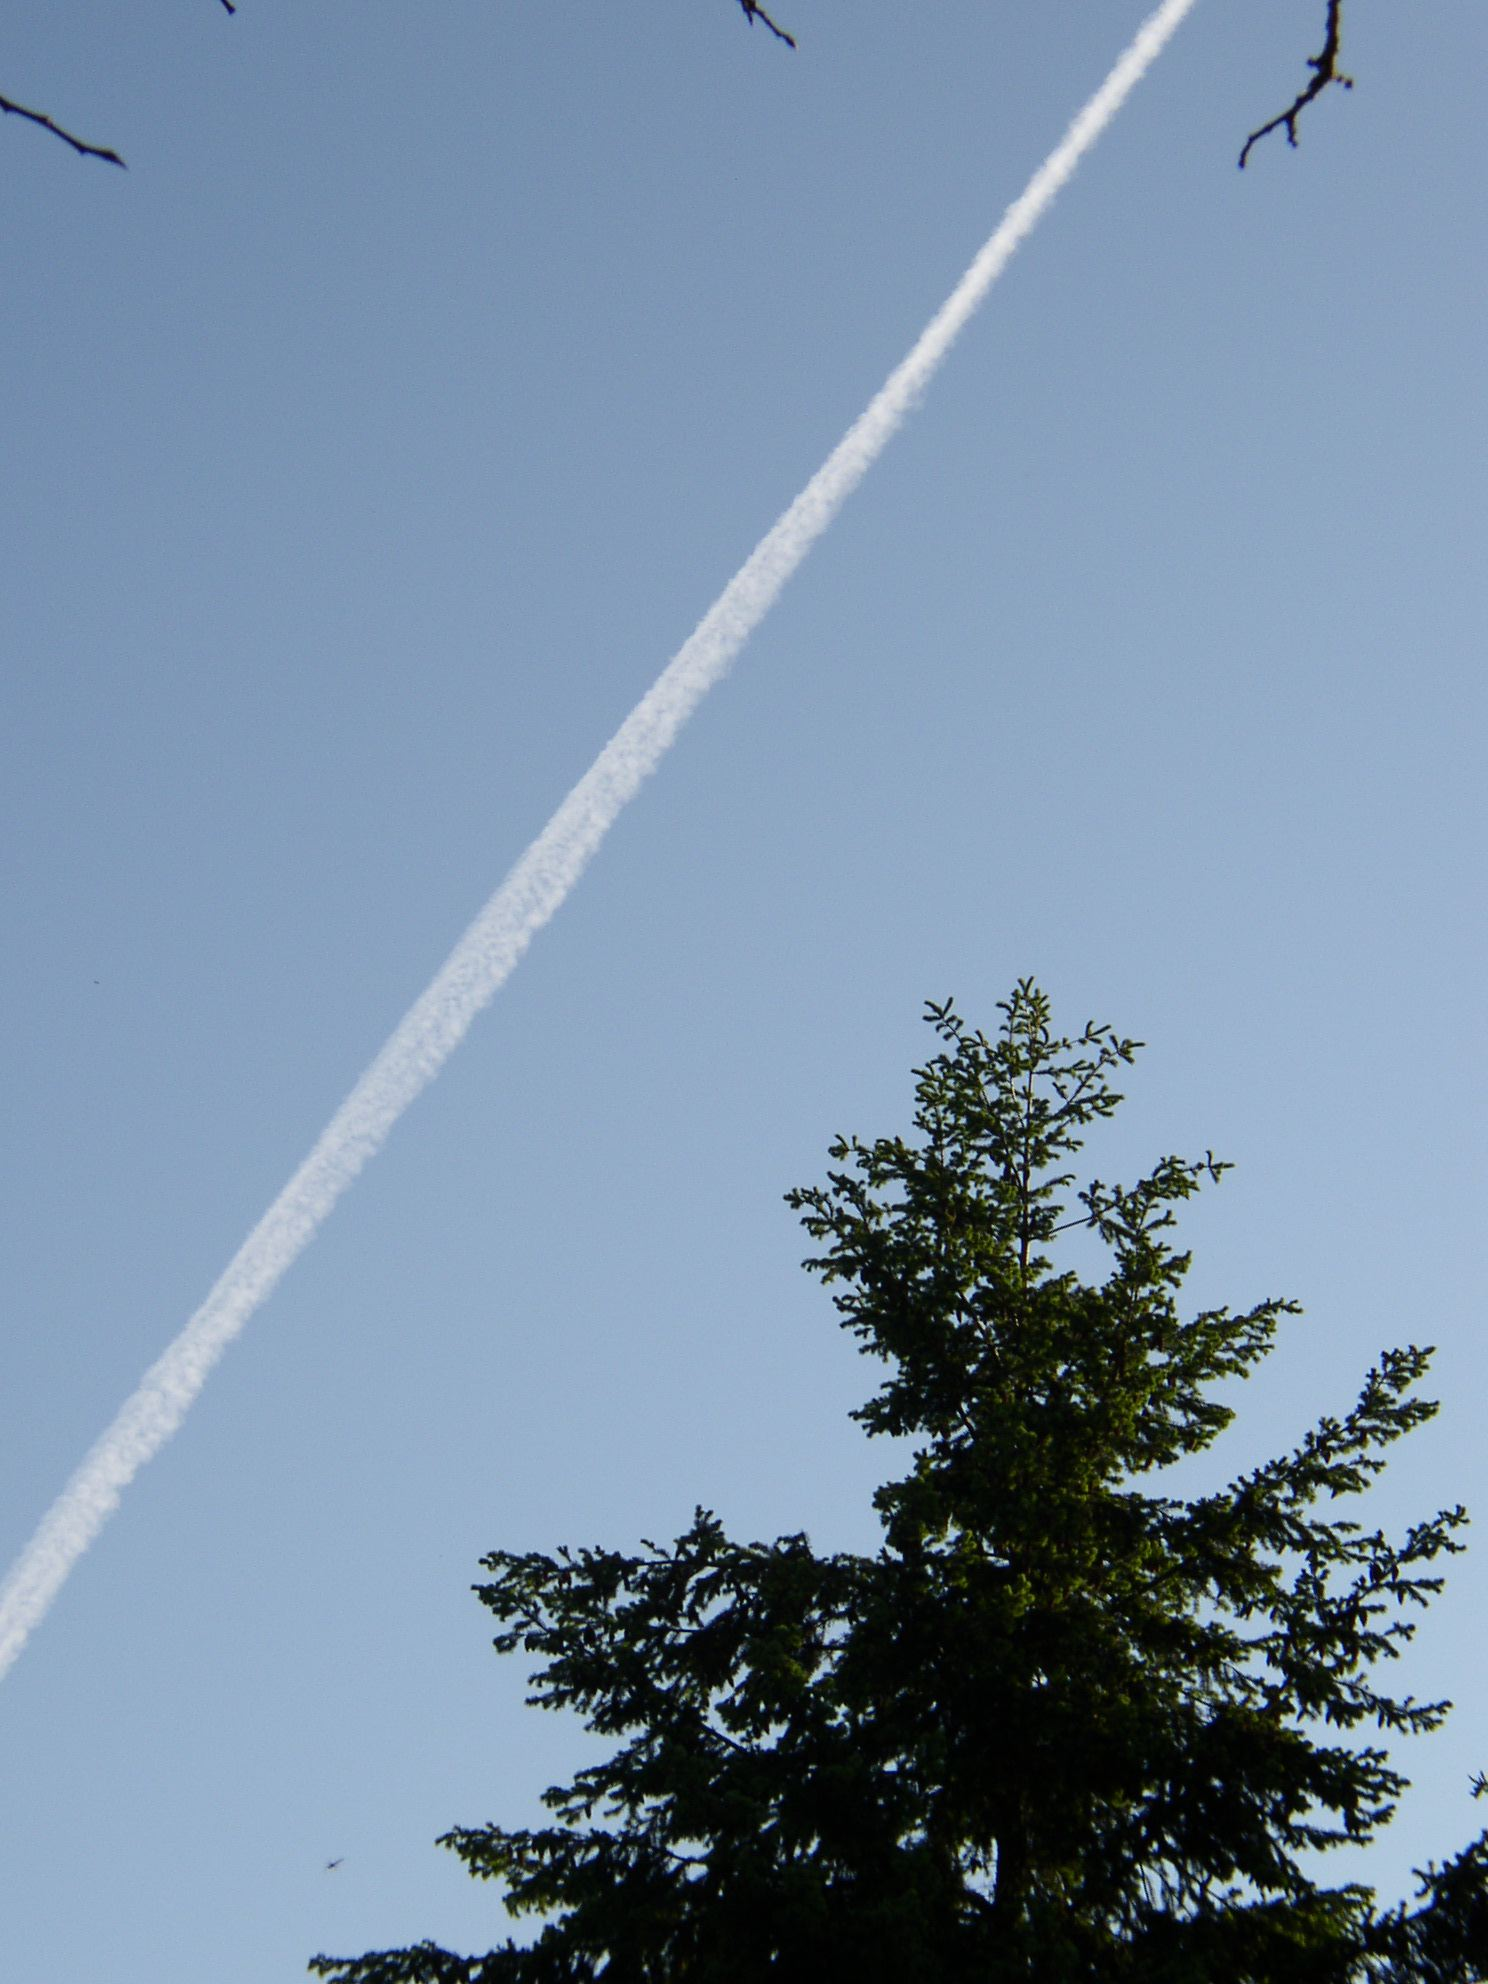
\includegraphics[width=3.0in]{pic/figure3.jpg}
\caption{Clear Sky with Contrails (1488 x 1984)}
\label{figure3}
\end{figure}

\begin{figure}[hbtp]
	\centering
	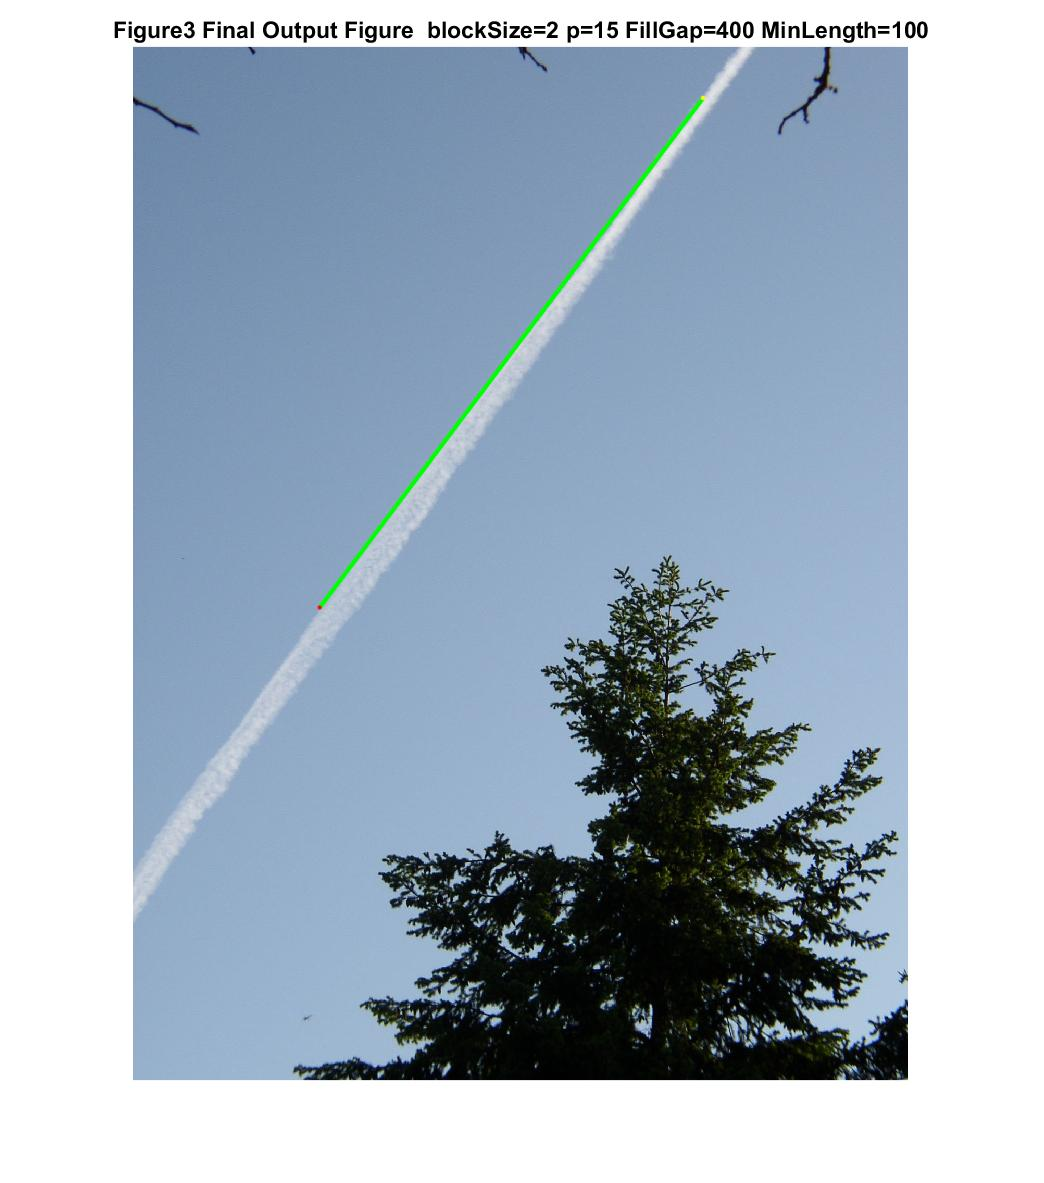
\includegraphics[width=6in]{pic/Figure3_best.jpg}
	\caption{Best Result for Figure \ref{figure3}}
	\label{Figure3_best}
\end{figure}


\begin{figure}[hbtp]
	\centering
	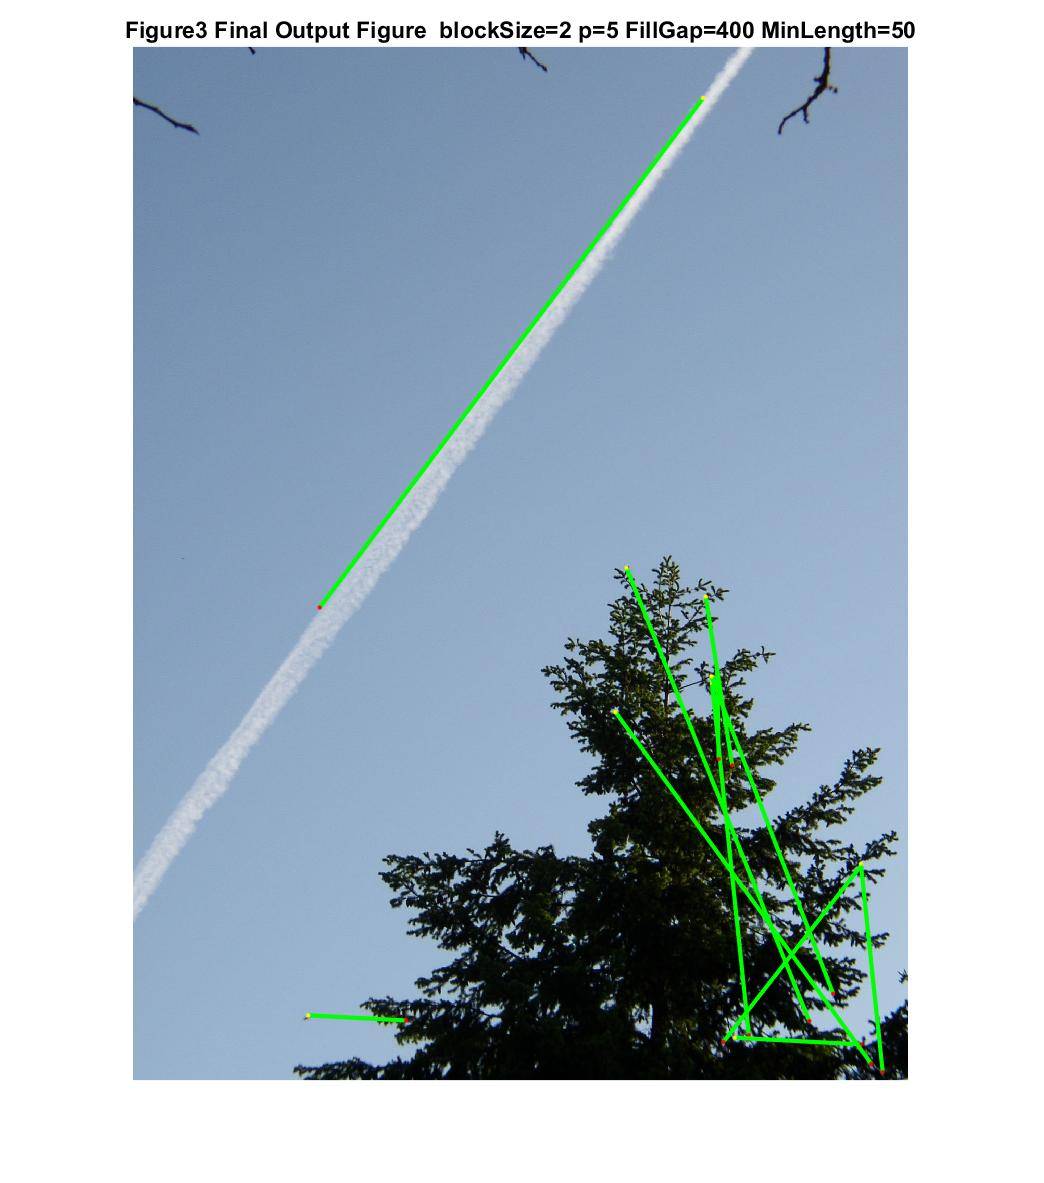
\includegraphics[width=6in]{pic/Figure3_worst.jpg}
	\caption{Worst Result for Figure \ref{figure3}, too many bad lines}
	\label{Figure3_worst}
\end{figure}

\clearpage
\begingroup
\setlength{\LTleft}{-20cm plus -1fill}
\setlength{\LTright}{\LTleft}
{\small
\begin{longtable}{| c | c | c | c | c | c | c | c | c |} \hline
Block & Percentage & FillGap & Minimum & Correct & Incorrect & Missingr & Correct & Incorrect \\
Radius &  & & Length & Number & Number & Number & Rate & Rate \\ \hline
12 & 5 & 200 & 50 & 2 & 0 & -1 & 200.00\% & 0.00\% \\
2 & 15 & 200 & 50 & 2 & 0 & -1 & 200.00\% & 0.00\% \\
2 & 15 & 200 & 100 & 2 & 0 & -1 & 200.00\% & 0.00\% \\
2 & 25 & 200 & 50 & 2 & 0 & -1 & 200.00\% & 0.00\% \\
2 & 25 & 200 & 100 & 2 & 0 & -1 & 200.00\% & 0.00\% \\
2 & 15 & 200 & 25 & 2 & 0 & -1 & 200.00\% & 0.00\% \\
2 & 25 & 200 & 25 & 2 & 0 & -1 & 200.00\% & 0.00\% \\
7 & 5 & 200 & 100 & 2 & 0 & -1 & 200.00\% & 0.00\% \\
7 & 15 & 200 & 50 & 2 & 0 & -1 & 200.00\% & 0.00\% \\
7 & 15 & 200 & 100 & 2 & 0 & -1 & 200.00\% & 0.00\% \\
7 & 25 & 200 & 50 & 2 & 0 & -1 & 200.00\% & 0.00\% \\
7 & 25 & 200 & 100 & 2 & 0 & -1 & 200.00\% & 0.00\% \\
7 & 5 & 200 & 25 & 2 & 0 & -1 & 200.00\% & 0.00\% \\
7 & 15 & 200 & 25 & 2 & 0 & -1 & 200.00\% & 0.00\% \\
7 & 25 & 200 & 25 & 2 & 0 & -1 & 200.00\% & 0.00\% \\
12 & 5 & 200 & 100 & 2 & 0 & -1 & 200.00\% & 0.00\% \\
12 & 15 & 200 & 50 & 2 & 0 & -1 & 200.00\% & 0.00\% \\
12 & 15 & 200 & 100 & 2 & 0 & -1 & 200.00\% & 0.00\% \\
12 & 25 & 200 & 50 & 2 & 0 & -1 & 200.00\% & 0.00\% \\
12 & 25 & 200 & 100 & 2 & 0 & -1 & 200.00\% & 0.00\% \\
12 & 5 & 200 & 25 & 2 & 0 & -1 & 200.00\% & 0.00\% \\
12 & 15 & 200 & 25 & 2 & 0 & -1 & 200.00\% & 0.00\% \\
12 & 25 & 200 & 25 & 2 & 0 & -1 & 200.00\% & 0.00\% \\
7 & 5 & 200 & 50 & 2 & 0 & -1 & 200.00\% & 0.00\% \\
2 & 5 & 200 & 100 & 2 & 6 & -1 & 200.00\% & 75.00\% \\
2 & 5 & 200 & 25 & 2 & 7 & -1 & 200.00\% & 77.78\% \\
2 & 5 & 200 & 50 & 2 & 7 & -1 & 200.00\% & 77.78\% \\
2 & 15 & 400 & 25 & 1 & 0 & 0 & 100.00\% & 0.00\% \\
2 & 25 & 400 & 25 & 1 & 0 & 0 & 100.00\% & 0.00\% \\
2 & 15 & 400 & 50 & 1 & 0 & 0 & 100.00\% & 0.00\% \\
2 & 15 & 400 & 100 & 1 & 0 & 0 & 100.00\% & 0.00\% \\
2 & 15 & 600 & 25 & 1 & 0 & 0 & 100.00\% & 0.00\% \\
2 & 15 & 600 & 50 & 1 & 0 & 0 & 100.00\% & 0.00\% \\
2 & 15 & 600 & 100 & 1 & 0 & 0 & 100.00\% & 0.00\% \\
2 & 25 & 400 & 50 & 1 & 0 & 0 & 100.00\% & 0.00\% \\
2 & 25 & 400 & 100 & 1 & 0 & 0 & 100.00\% & 0.00\% \\
2 & 25 & 600 & 25 & 1 & 0 & 0 & 100.00\% & 0.00\% \\
2 & 25 & 600 & 50 & 1 & 0 & 0 & 100.00\% & 0.00\% \\
2 & 25 & 600 & 100 & 1 & 0 & 0 & 100.00\% & 0.00\% \\
7 & 15 & 400 & 25 & 1 & 0 & 0 & 100.00\% & 0.00\% \\
7 & 25 & 400 & 25 & 1 & 0 & 0 & 100.00\% & 0.00\% \\
7 & 5 & 400 & 50 & 1 & 0 & 0 & 100.00\% & 0.00\% \\
7 & 5 & 400 & 100 & 1 & 0 & 0 & 100.00\% & 0.00\% \\
7 & 5 & 600 & 25 & 1 & 0 & 0 & 100.00\% & 0.00\% \\
7 & 5 & 600 & 50 & 1 & 0 & 0 & 100.00\% & 0.00\% \\
7 & 5 & 600 & 100 & 1 & 0 & 0 & 100.00\% & 0.00\% \\
7 & 15 & 400 & 50 & 1 & 0 & 0 & 100.00\% & 0.00\% \\
7 & 15 & 400 & 100 & 1 & 0 & 0 & 100.00\% & 0.00\% \\
7 & 15 & 600 & 25 & 1 & 0 & 0 & 100.00\% & 0.00\% \\
7 & 15 & 600 & 50 & 1 & 0 & 0 & 100.00\% & 0.00\% \\
7 & 15 & 600 & 100 & 1 & 0 & 0 & 100.00\% & 0.00\% \\
7 & 25 & 400 & 50 & 1 & 0 & 0 & 100.00\% & 0.00\% \\
7 & 25 & 400 & 100 & 1 & 0 & 0 & 100.00\% & 0.00\% \\
7 & 25 & 600 & 25 & 1 & 0 & 0 & 100.00\% & 0.00\% \\
7 & 25 & 600 & 50 & 1 & 0 & 0 & 100.00\% & 0.00\% \\
7 & 25 & 600 & 100 & 1 & 0 & 0 & 100.00\% & 0.00\% \\
12 & 15 & 400 & 25 & 1 & 0 & 0 & 100.00\% & 0.00\% \\
12 & 25 & 400 & 25 & 1 & 0 & 0 & 100.00\% & 0.00\% \\
12 & 5 & 400 & 50 & 1 & 0 & 0 & 100.00\% & 0.00\% \\
12 & 5 & 400 & 100 & 1 & 0 & 0 & 100.00\% & 0.00\% \\
12 & 5 & 600 & 25 & 1 & 0 & 0 & 100.00\% & 0.00\% \\
12 & 5 & 600 & 50 & 1 & 0 & 0 & 100.00\% & 0.00\% \\
12 & 5 & 600 & 100 & 1 & 0 & 0 & 100.00\% & 0.00\% \\
12 & 15 & 400 & 50 & 1 & 0 & 0 & 100.00\% & 0.00\% \\
12 & 15 & 400 & 100 & 1 & 0 & 0 & 100.00\% & 0.00\% \\
12 & 15 & 600 & 25 & 1 & 0 & 0 & 100.00\% & 0.00\% \\
12 & 15 & 600 & 50 & 1 & 0 & 0 & 100.00\% & 0.00\% \\
12 & 15 & 600 & 100 & 1 & 0 & 0 & 100.00\% & 0.00\% \\
12 & 25 & 400 & 50 & 1 & 0 & 0 & 100.00\% & 0.00\% \\
12 & 25 & 400 & 100 & 1 & 0 & 0 & 100.00\% & 0.00\% \\
12 & 25 & 600 & 25 & 1 & 0 & 0 & 100.00\% & 0.00\% \\
12 & 25 & 600 & 50 & 1 & 0 & 0 & 100.00\% & 0.00\% \\
12 & 25 & 600 & 100 & 1 & 0 & 0 & 100.00\% & 0.00\% \\
7 & 5 & 400 & 25 & 1 & 0 & 0 & 100.00\% & 0.00\% \\
12 & 5 & 400 & 25 & 1 & 0 & 0 & 100.00\% & 0.00\% \\
2 & 5 & 400 & 25 & 1 & 6 & 0 & 100.00\% & 85.71\% \\
2 & 5 & 400 & 50 & 1 & 6 & 0 & 100.00\% & 85.71\% \\
2 & 5 & 400 & 100 & 1 & 6 & 0 & 100.00\% & 85.71\% \\
2 & 5 & 600 & 25 & 1 & 6 & 0 & 100.00\% & 85.71\% \\
2 & 5 & 600 & 50 & 1 & 6 & 0 & 100.00\% & 85.71\% \\
2 & 5 & 600 & 100 & 1 & 6 & 0 & 100.00\% & 85.71\% \\ \\\hline
\caption{Experimental results for Figure \ref{figure3}.}
\label{table3}
\end{longtable}
}
\endgroup



\clearpage
\subsection{Aerial Image}

Figure \ref{figure4} is a colored aerial image with about too many contrails which are hard to be clear recognized and counted. These contrails cross each other, and most of them are all thin and blurry. According to the rule 4 above, we count it as 10, for it is so difficult to find out the actual number. \\
The best result has the parameters with block radius as 2, percentage to keep as 15, fill gap as 600, and minimum length can be any in 25, 50 and 100. The best result covers more than half of the contrails on the image. Anyway, because too many unclear contrails exist on the image, and the default contrails to find is only 10, we cannot find all the contrails. And the worst one covers very few contrails on the image with most confused thing is the results lines are parallel or perpendicular with each other. The results image for figure \ref{figure4} can be seen at figure \ref{Figure4_best} for the best result and figure \ref{Figure4_worst} for the worst result.

\begin{figure}[htb!]
\centering
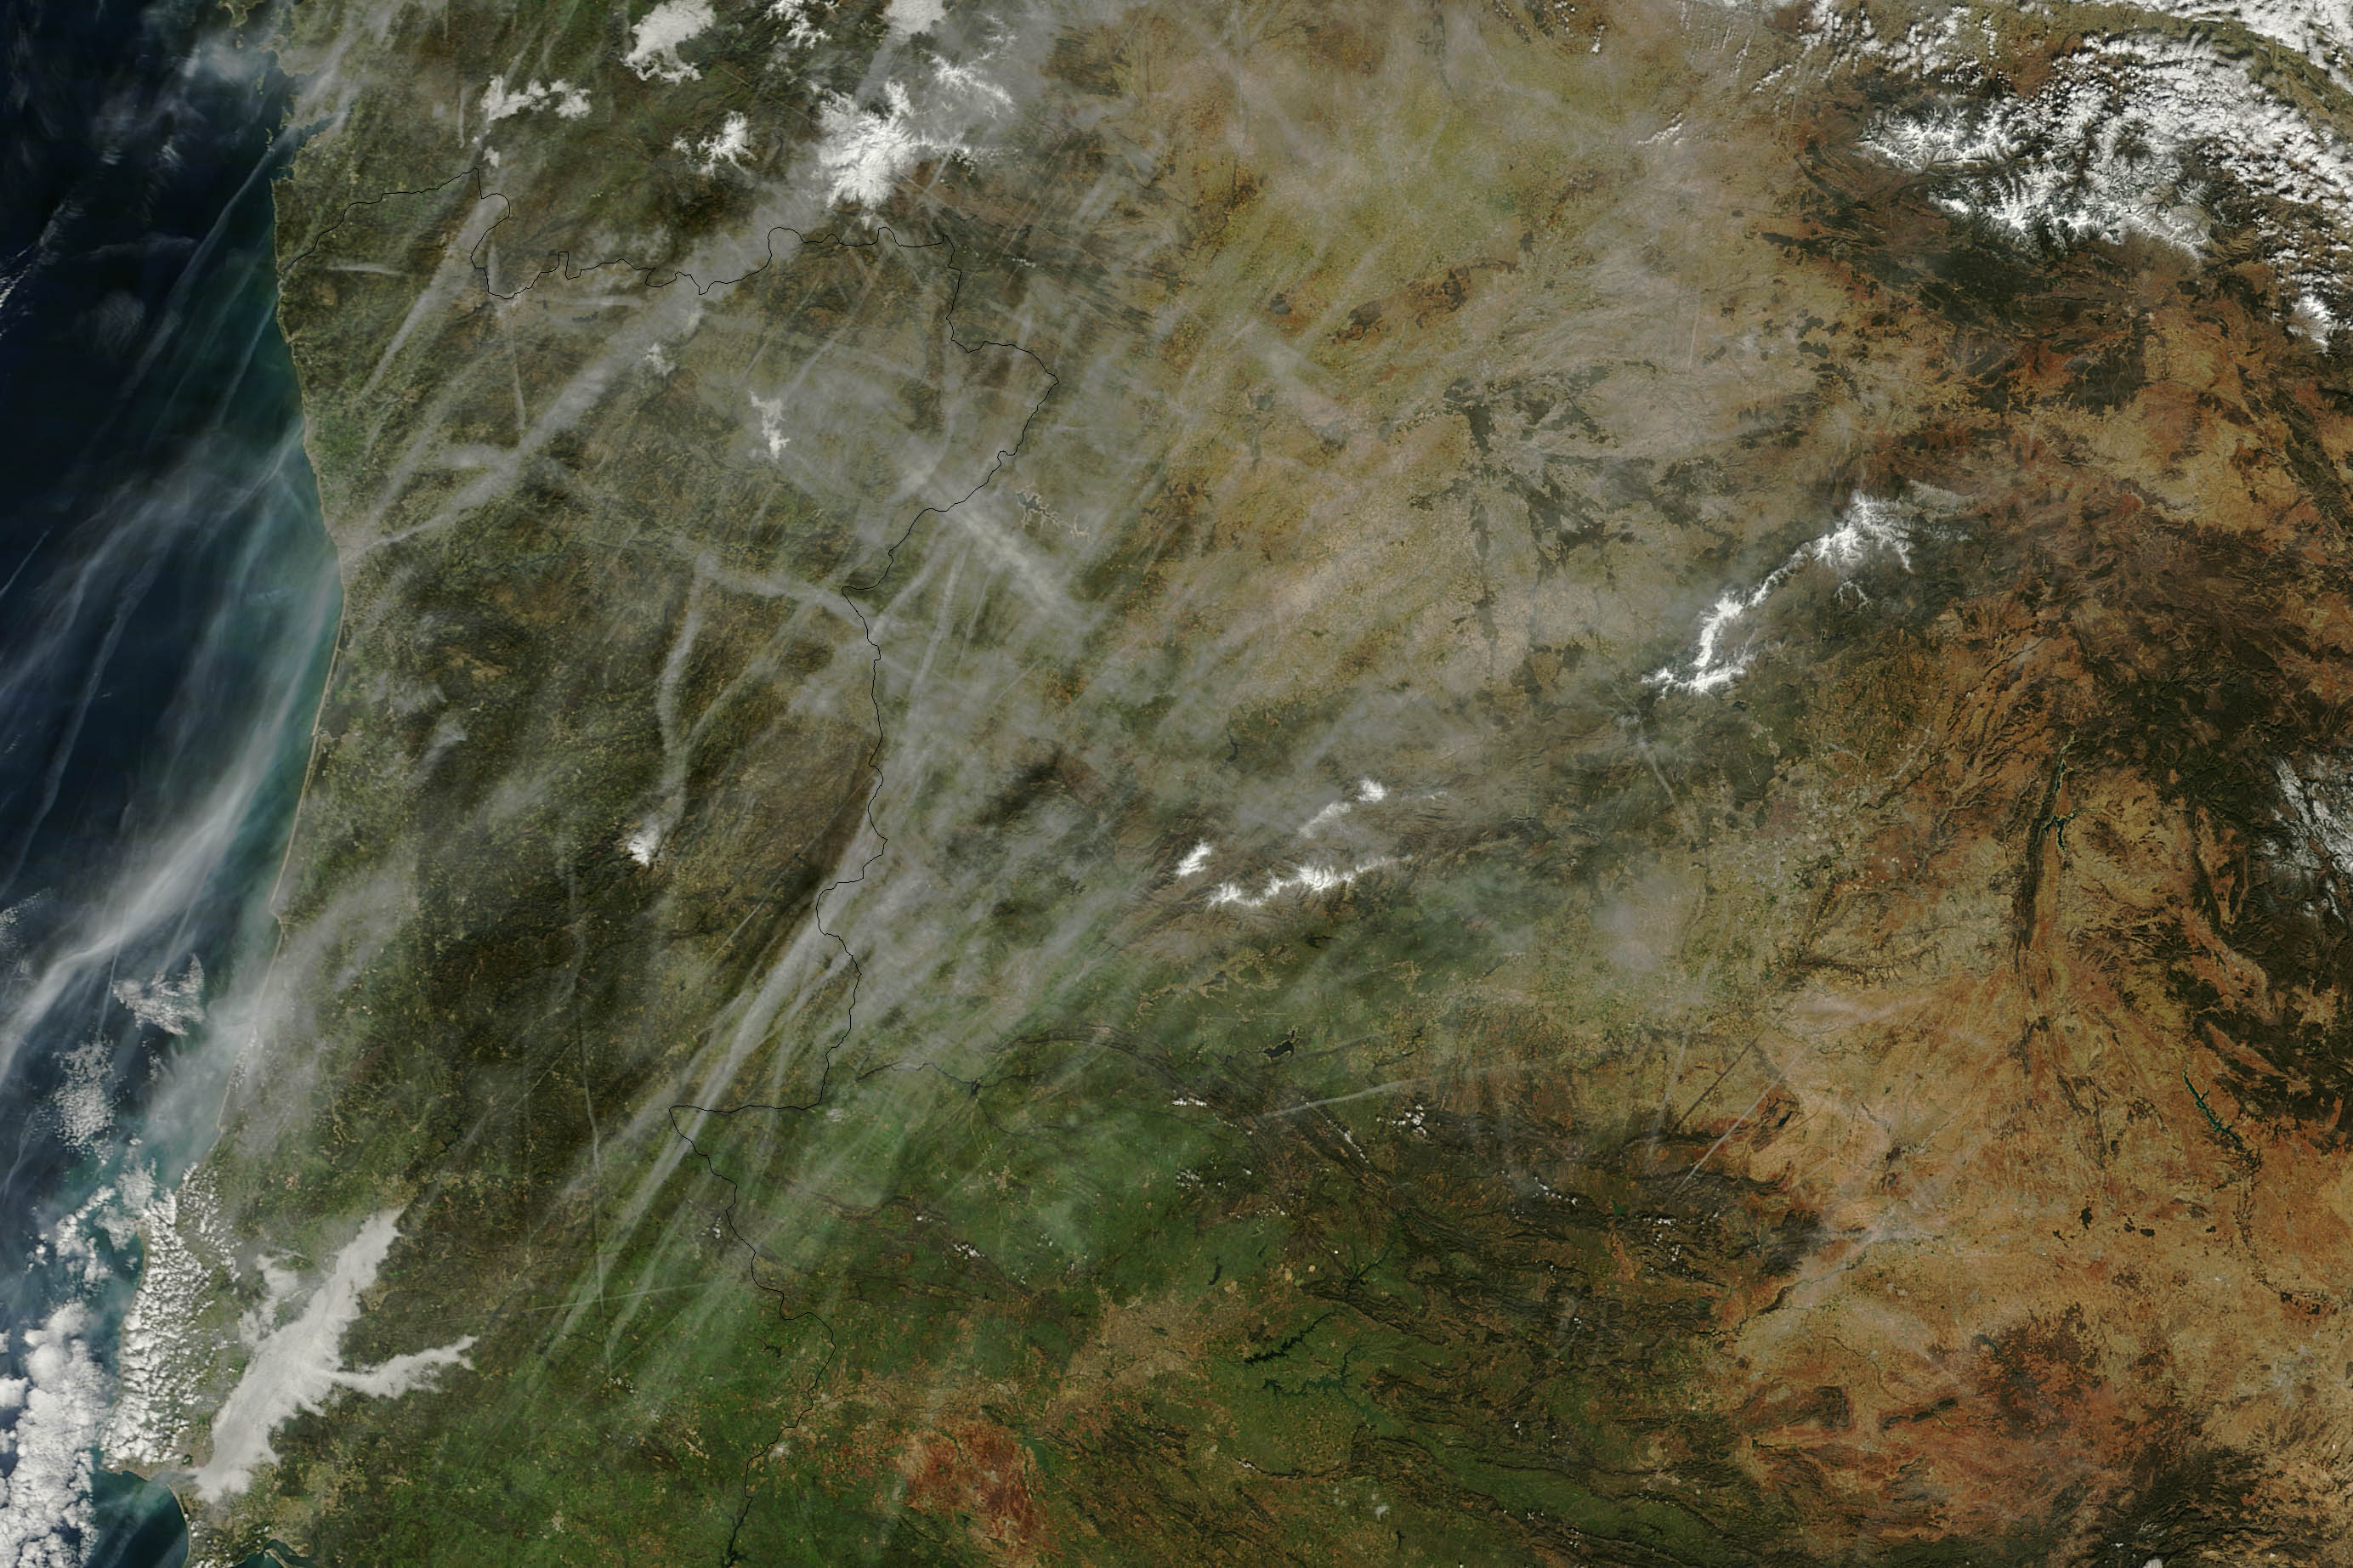
\includegraphics[width=6in]{pic/figure4.jpg}
\caption{Aerial Image (2768 x 1845)}
\label{figure4}
\end{figure}

\begin{figure}[hbtp]
	\centering
	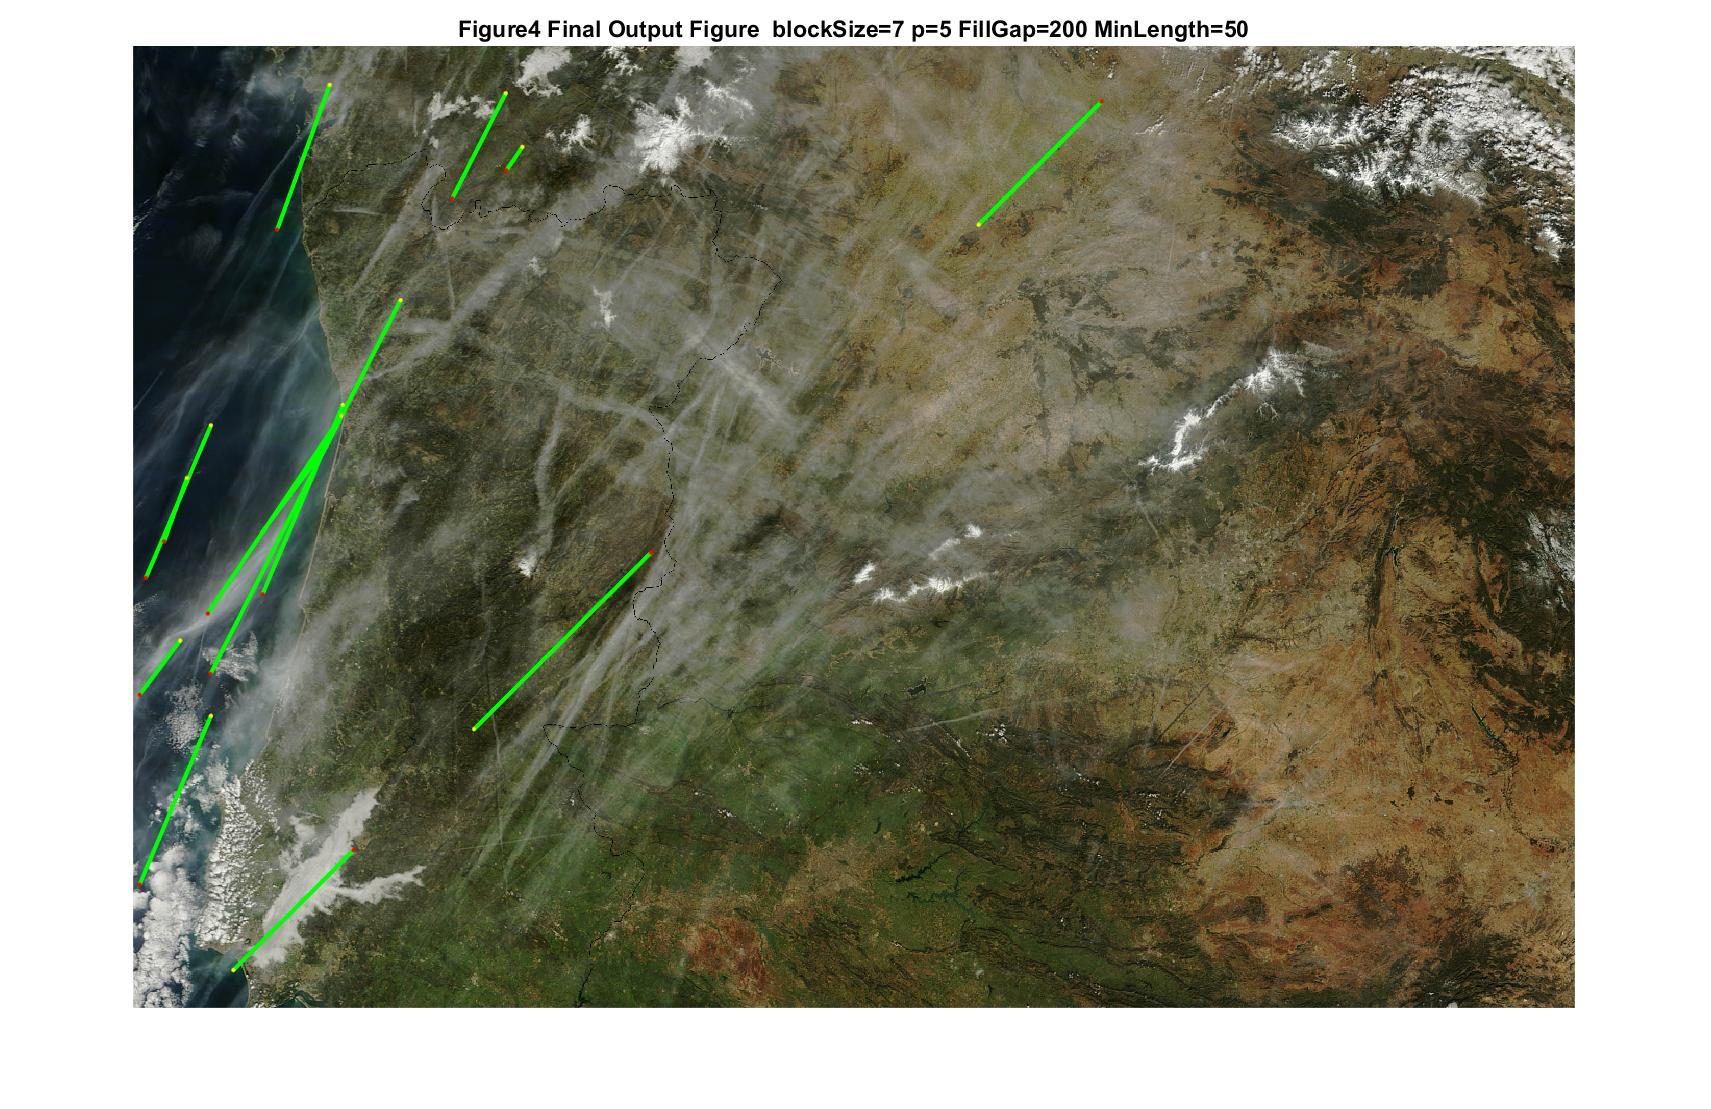
\includegraphics[width=6in]{pic/Figure4_best.jpg}
	\caption{Best Result for Figure \ref{figure4}}
	\label{Figure4_best}
\end{figure}


\begin{figure}[hbtp]
	\centering
	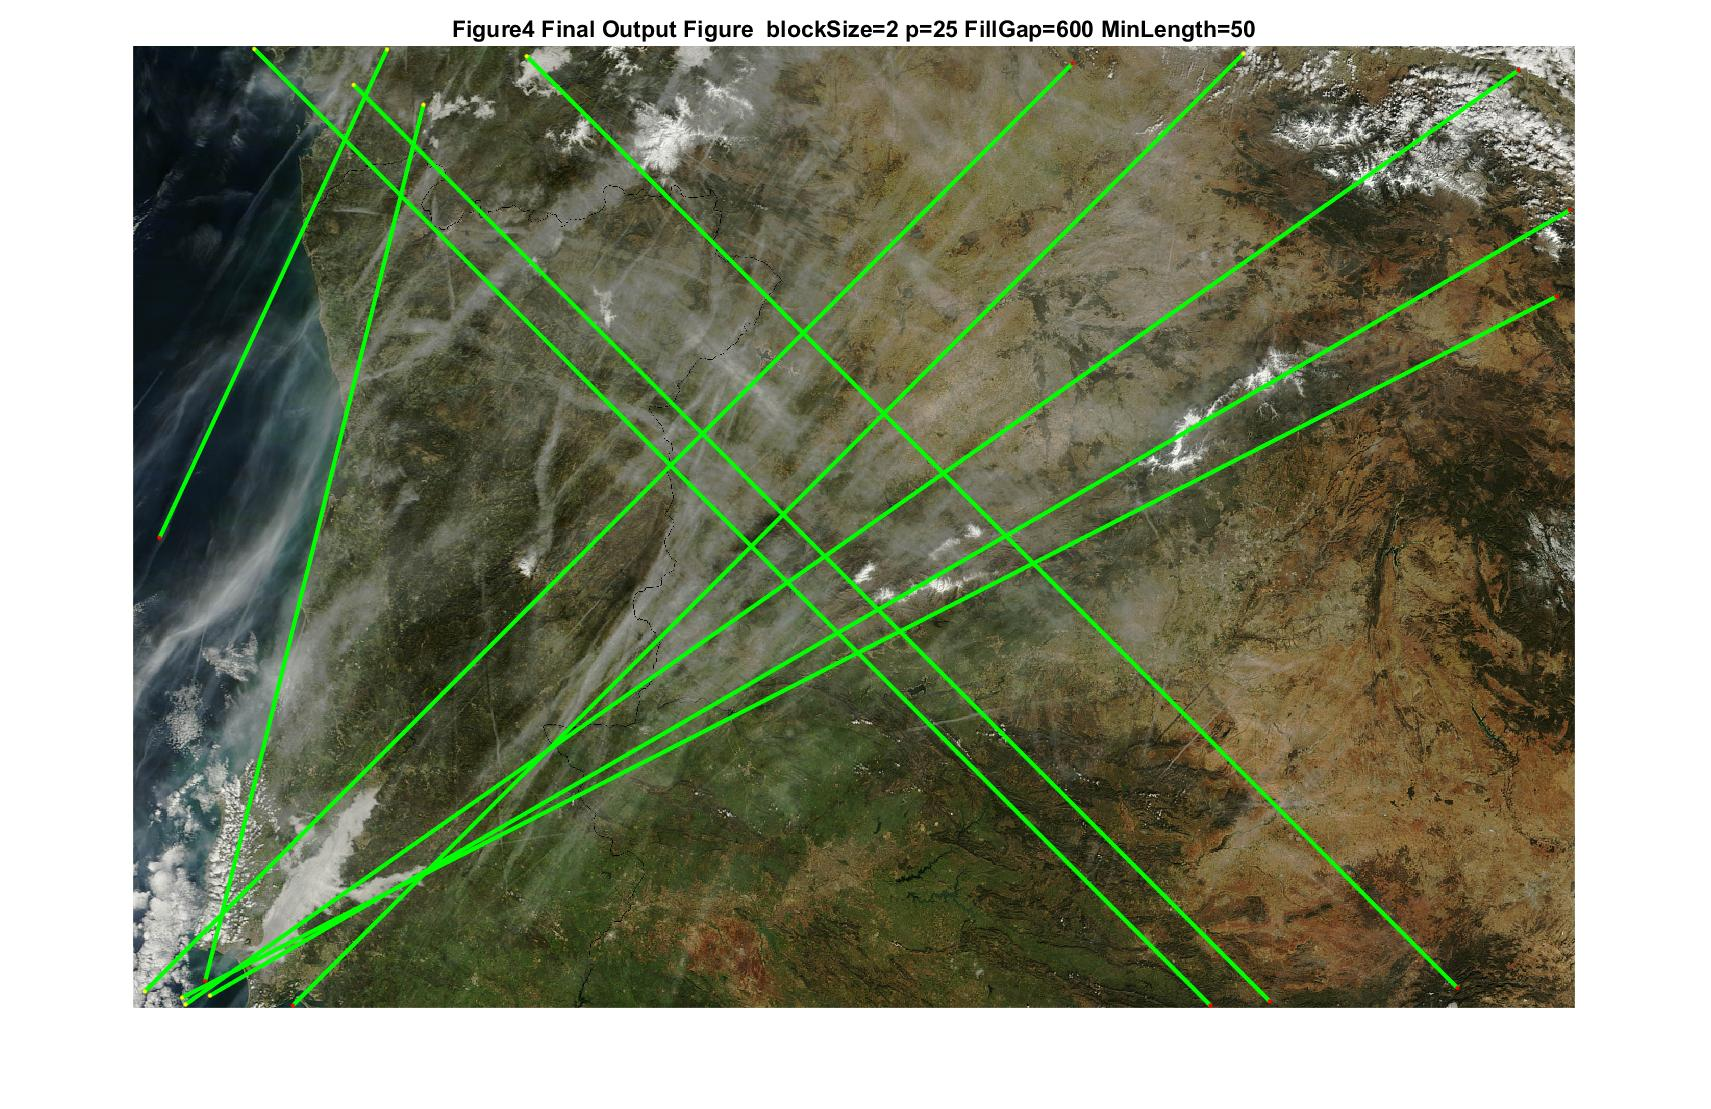
\includegraphics[width=6in]{pic/Figure4_worst.jpg}
	\caption{Worst Result for Figure \ref{figure4}, lines parallel or perpendicular}
	\label{Figure4_worst}
\end{figure}

\clearpage
\begingroup
\setlength{\LTleft}{-20cm plus -1fill}
\setlength{\LTright}{\LTleft}
{\small
\begin{longtable}{| c | c | c | c | c | c | c | c | c |} \hline
Block & Percentage & FillGap & Minimum & Correct & Incorrect & Missingr & Correct & Incorrect \\
Radius &  & & Length & Number & Number & Number & Rate & Rate \\ \hline
7&5&200&50&6&3&4&60.00\%&33.33\%\\
7&5&200&25&6&4&4&60.00\%&40.00\%\\
2&15&200&25&4&1&6&40.00\%&20.00\%\\
2&15&200&50&4&1&6&40.00\%&20.00\%\\
2&15&200&100&4&1&6&40.00\%&20.00\%\\
2&15&400&25&3&0&7&30.00\%&0.00\%\\
2&15&400&50&3&0&7&30.00\%&0.00\%\\
2&15&400&100&3&0&7&30.00\%&0.00\%\\
2&15&600&25&3&0&7&30.00\%&0.00\%\\
2&15&600&50&3&0&7&30.00\%&0.00\%\\
2&15&600&100&3&0&7&30.00\%&0.00\%\\
7&5&400&25&3&1&7&30.00\%&25.00\%\\
7&5&400&50&3&1&7&30.00\%&25.00\%\\
7&5&400&100&3&1&7&30.00\%&25.00\%\\
7&5&600&25&3&1&7&30.00\%&25.00\%\\
7&5&600&50&3&1&7&30.00\%&25.00\%\\
7&5&600&100&3&1&7&30.00\%&25.00\%\\
2&25&200&25&3&8&7&30.00\%&72.73\%\\
2&25&200&50&3&8&7&30.00\%&72.73\%\\
2&25&200&100&3&8&7&30.00\%&72.73\%\\
12&5&200&50&2&2&8&20.00\%&50.00\%\\
12&5&200&100&2&2&8&20.00\%&50.00\%\\
12&5&400&25&2&2&8&20.00\%&50.00\%\\
12&5&400&50&2&2&8&20.00\%&50.00\%\\
12&5&400&100&2&2&8&20.00\%&50.00\%\\
12&5&600&25&2&2&8&20.00\%&50.00\%\\
12&5&600&50&2&2&8&20.00\%&50.00\%\\
12&5&600&100&2&2&8&20.00\%&50.00\%\\
12&5&200&25&2&3&8&20.00\%&60.00\%\\
2&25&400&25&2&8&8&20.00\%&80.00\%\\
2&25&400&50&2&8&8&20.00\%&80.00\%\\
2&25&400&100&2&8&8&20.00\%&80.00\%\\
2&25&600&25&2&8&8&20.00\%&80.00\%\\
2&25&600&50&2&8&8&20.00\%&80.00\%\\
2&25&600&100&2&8&8&20.00\%&80.00\%\\
7&15&200&25&2&10&8&20.00\%&83.33\%\\
7&15&200&50&2&10&8&20.00\%&83.33\%\\
7&15&200&100&2&10&8&20.00\%&83.33\%\\
2&5&200&50&1&0&9&10.00\%&0.00\%\\
2&5&200&100&1&0&9&10.00\%&0.00\%\\
2&5&400&25&1&0&9&10.00\%&0.00\%\\
2&5&400&50&1&0&9&10.00\%&0.00\%\\
2&5&400&100&1&0&9&10.00\%&0.00\%\\
2&5&600&25&1&0&9&10.00\%&0.00\%\\
2&5&600&50&1&0&9&10.00\%&0.00\%\\
2&5&600&100&1&0&9&10.00\%&0.00\%\\
7&15&400&25&1&10&9&10.00\%&90.91\%\\
7&15&400&50&1&10&9&10.00\%&90.91\%\\
7&15&400&100&1&10&9&10.00\%&90.91\%\\
7&15&600&25&1&10&9&10.00\%&90.91\%\\
7&15&600&50&1&10&9&10.00\%&90.91\%\\
7&15&600&100&1&10&9&10.00\%&90.91\%\\
7&25&200&25&0&10&10&0.00\%&100.00\%\\
7&25&200&50&0&10&10&0.00\%&100.00\%\\
7&25&200&100&0&10&10&0.00\%&100.00\%\\
7&25&400&25&0&10&10&0.00\%&100.00\%\\
7&25&400&50&0&10&10&0.00\%&100.00\%\\
7&25&400&100&0&10&10&0.00\%&100.00\%\\
7&25&600&25&0&10&10&0.00\%&100.00\%\\
7&25&600&50&0&10&10&0.00\%&100.00\%\\
7&25&600&100&0&10&10&0.00\%&100.00\%\\
12&15&200&25&0&10&10&0.00\%&100.00\%\\
12&15&200&50&0&10&10&0.00\%&100.00\%\\
12&15&200&100&0&10&10&0.00\%&100.00\%\\
12&15&400&25&0&10&10&0.00\%&100.00\%\\
12&15&400&50&0&10&10&0.00\%&100.00\%\\
12&15&400&100&0&10&10&0.00\%&100.00\%\\
12&15&600&25&0&10&10&0.00\%&100.00\%\\
12&15&600&50&0&10&10&0.00\%&100.00\%\\
12&15&600&100&0&10&10&0.00\%&100.00\%\\
12&25&200&25&0&10&10&0.00\%&100.00\%\\
12&25&200&50&0&10&10&0.00\%&100.00\%\\
12&25&200&100&0&10&10&0.00\%&100.00\%\\
12&25&400&25&0&10&10&0.00\%&100.00\%\\
12&25&400&50&0&10&10&0.00\%&100.00\%\\
12&25&400&100&0&10&10&0.00\%&100.00\%\\
12&25&600&25&0&10&10&0.00\%&100.00\%\\
12&25&600&50&0&10&10&0.00\%&100.00\%\\
12&25&600&100&0&10&10&0.00\%&100.00\%\\
2&5&200&25&0&10&10&0.00\%&100.00\%\\ \\\hline
\caption{Experimental results for Figure \ref{figure4}.}
\label{table4}
\end{longtable}
}
\endgroup


\clearpage
\subsection{Line of Trees and Open Sky}

Figure \ref{figure5} is a color image with about 3 contrails which are easier to be recognized, and there exists an apparent road and trees whose edges are close to the straight line.\\
The best result has the parameters with block radius as 12, percentage to keep as 15, fill gap as 200, and minimum length as 100. The best result cover the contrail, however, it doesn’t avoid the highway line in the bottom because its edge is much clear than contrails. And the worst one only covers the highway line in the bottom but no contrails. The results image for figure \ref{figure5} can be seen at figure \ref{Figure5_best} for the best result and figure \ref{Figure5_worst} for the worst result.

\begin{figure}[htb!]
\centering
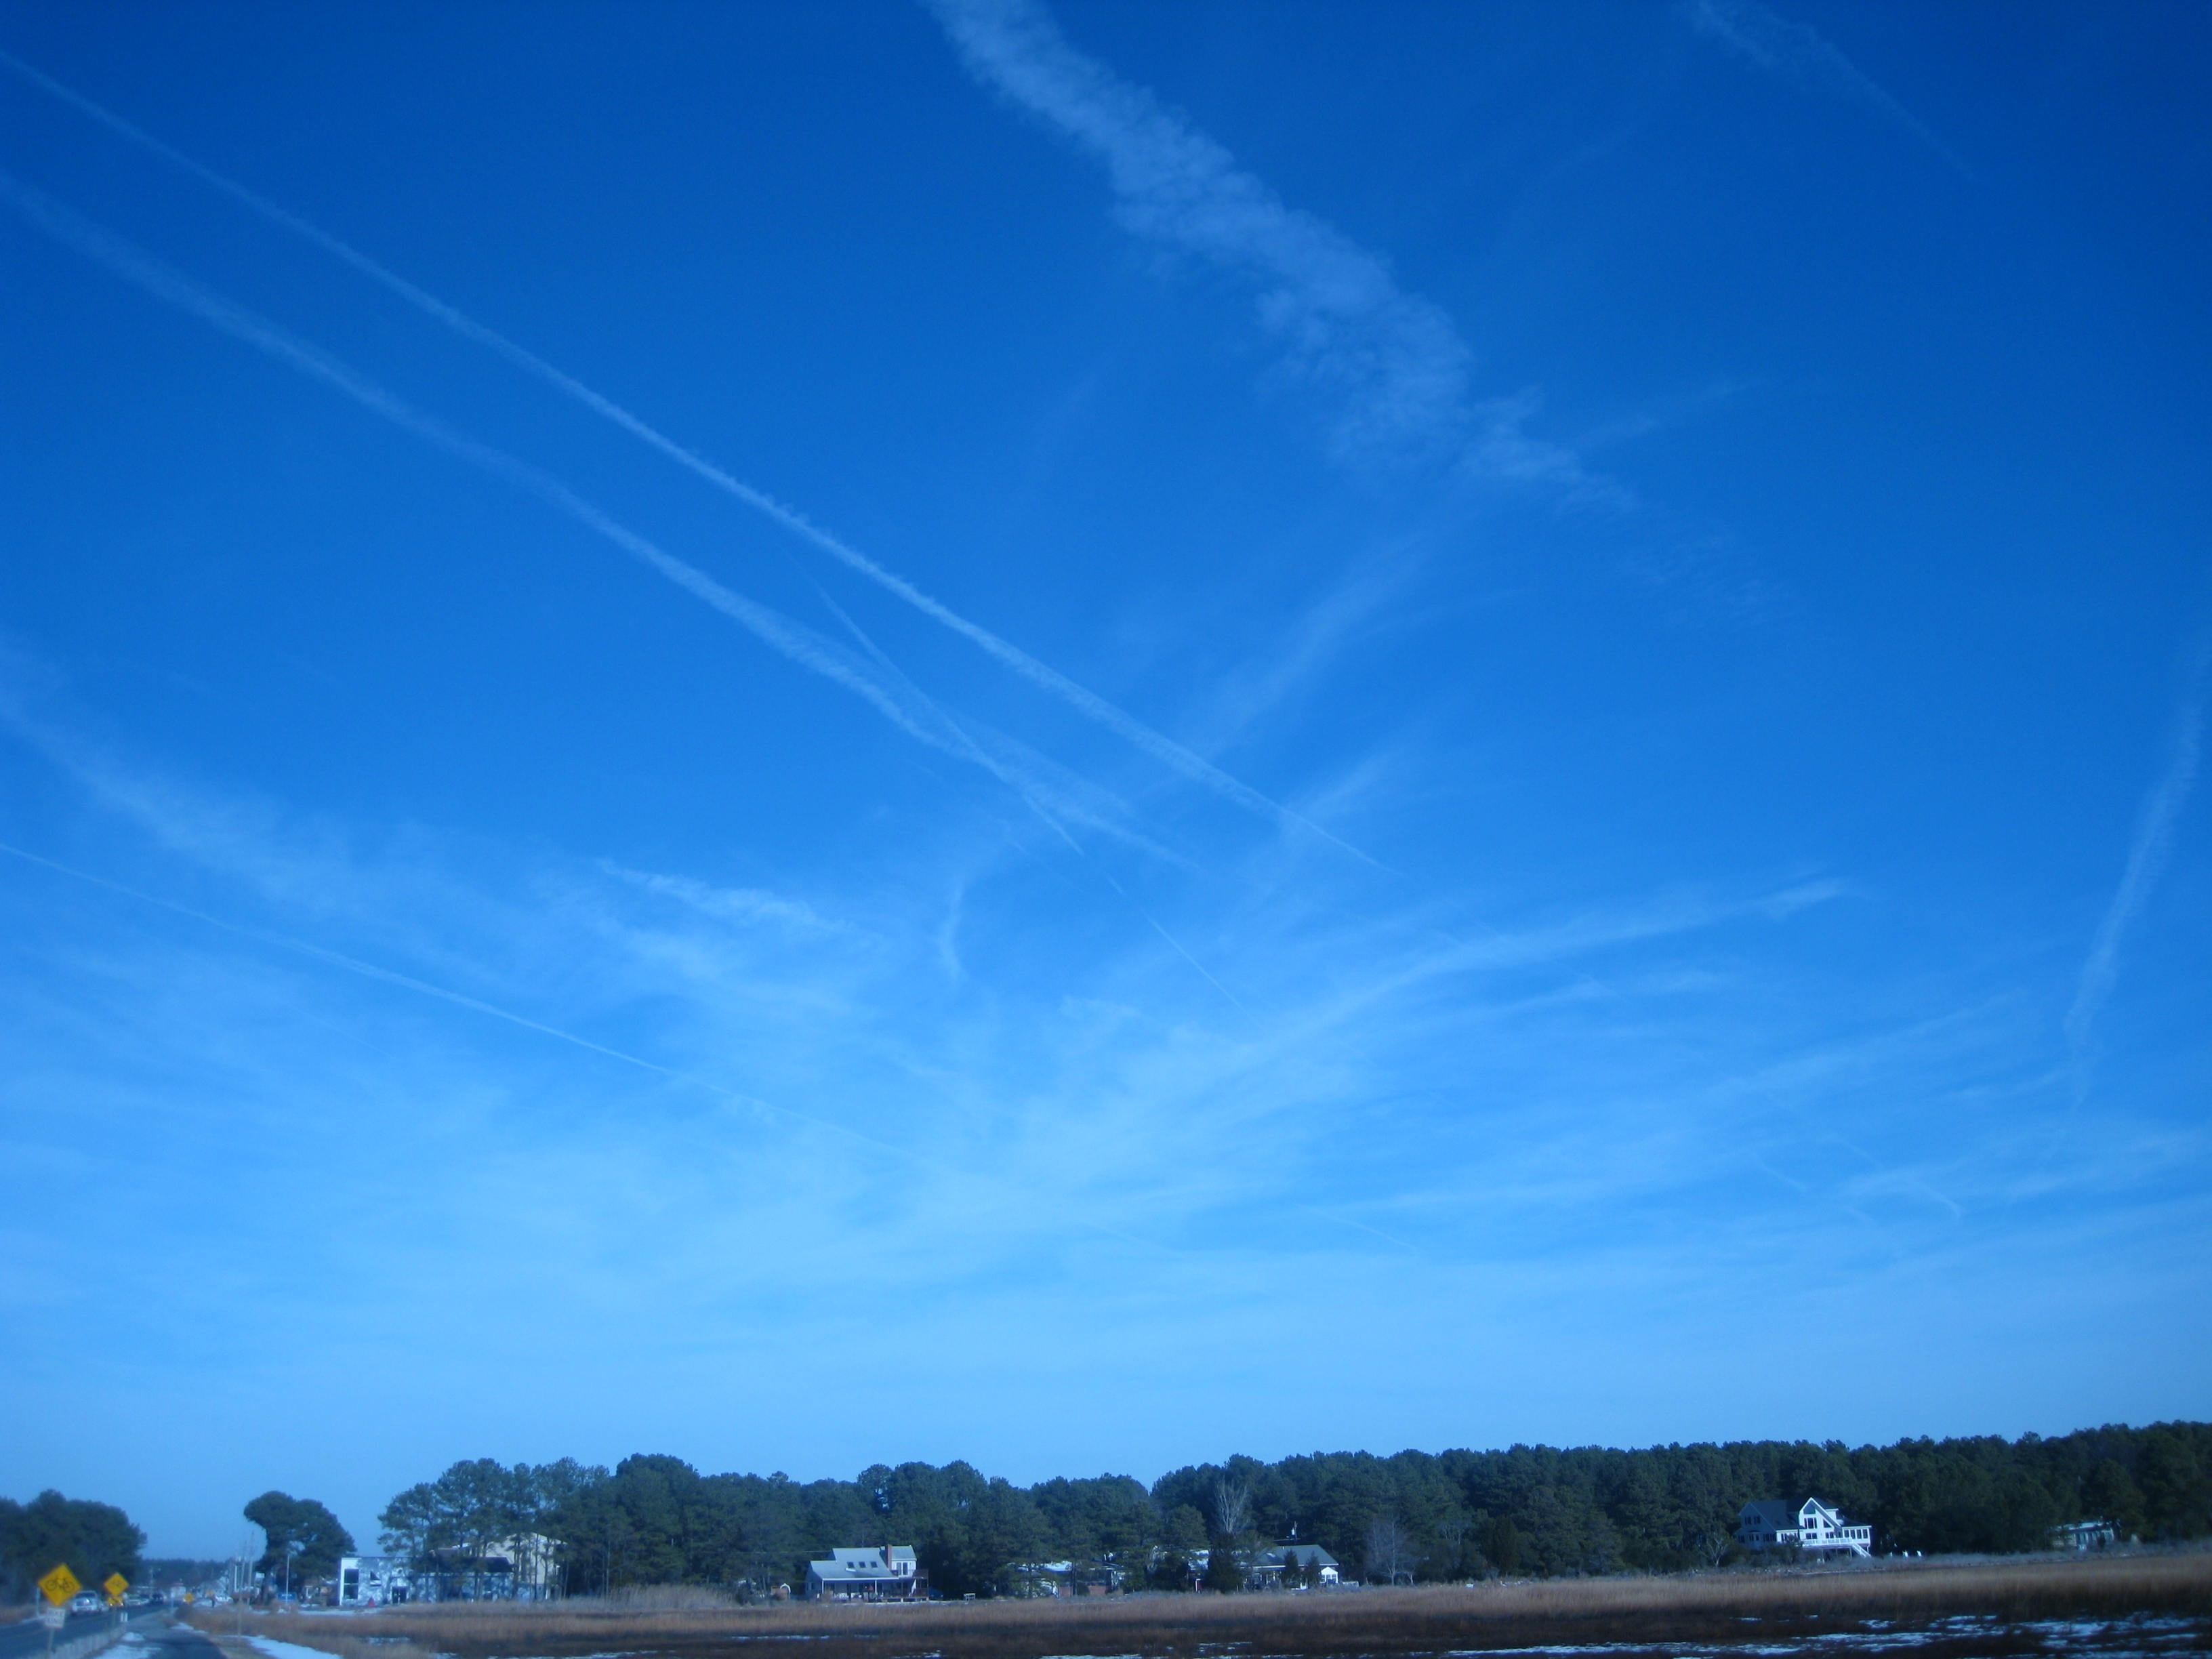
\includegraphics[width=6in]{pic/figure5.jpg}
\caption{Line of Trees and Open Sky (3264x2448)}
\label{figure5}
\end{figure}

\begin{figure}[hbtp]
	\centering
	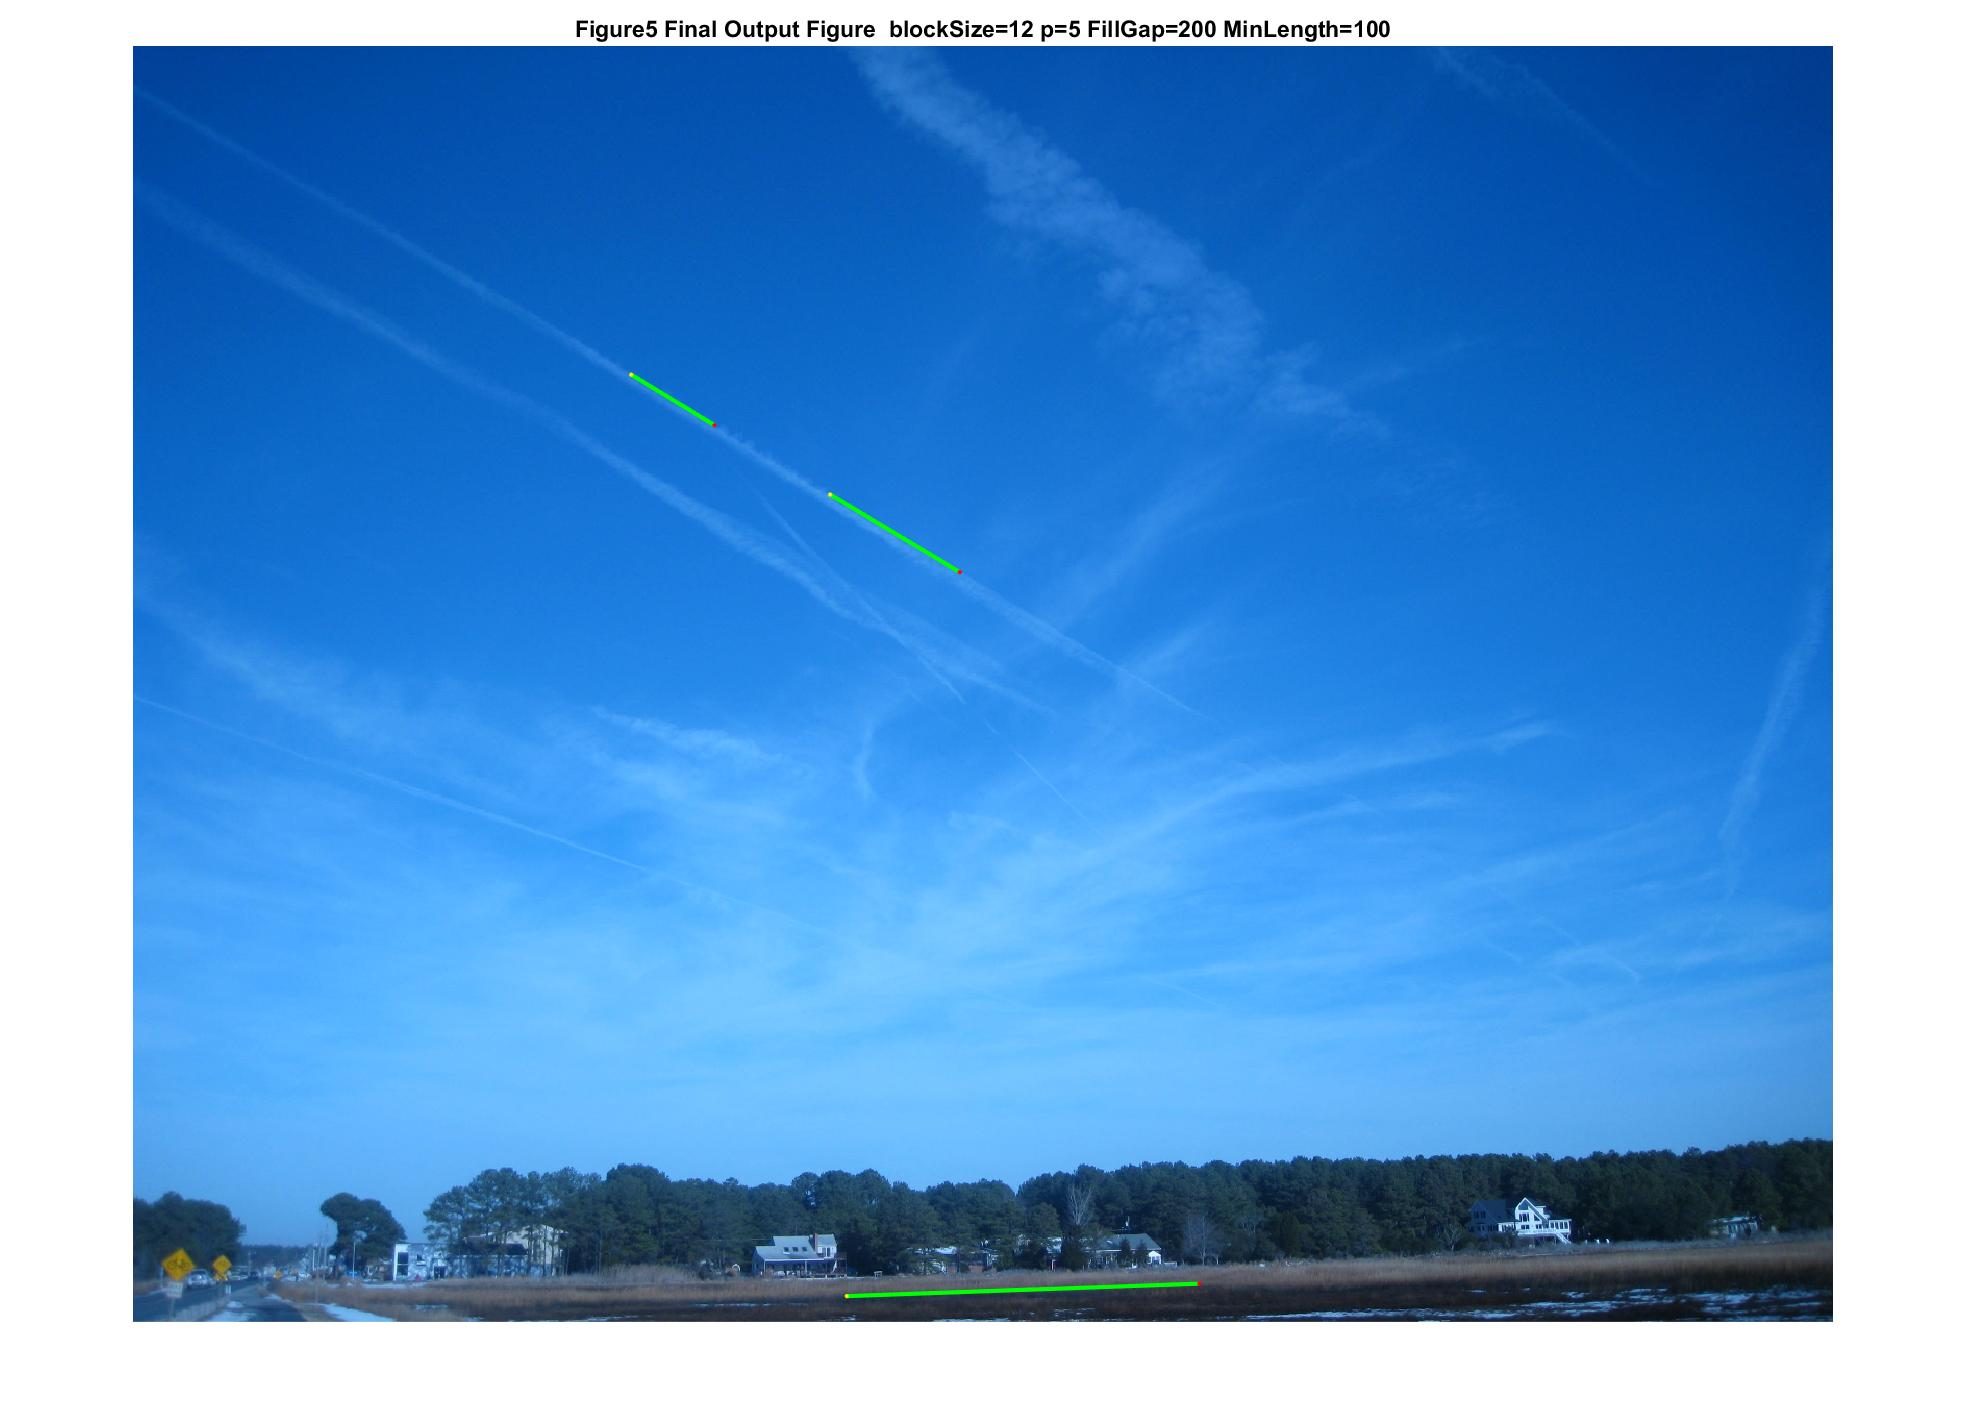
\includegraphics[width=6in]{pic/Figure5_best.jpg}
	\caption{Best Result for Figure \ref{figure5}}
	\label{Figure5_best}
\end{figure}


\begin{figure}[hbtp]
	\centering
	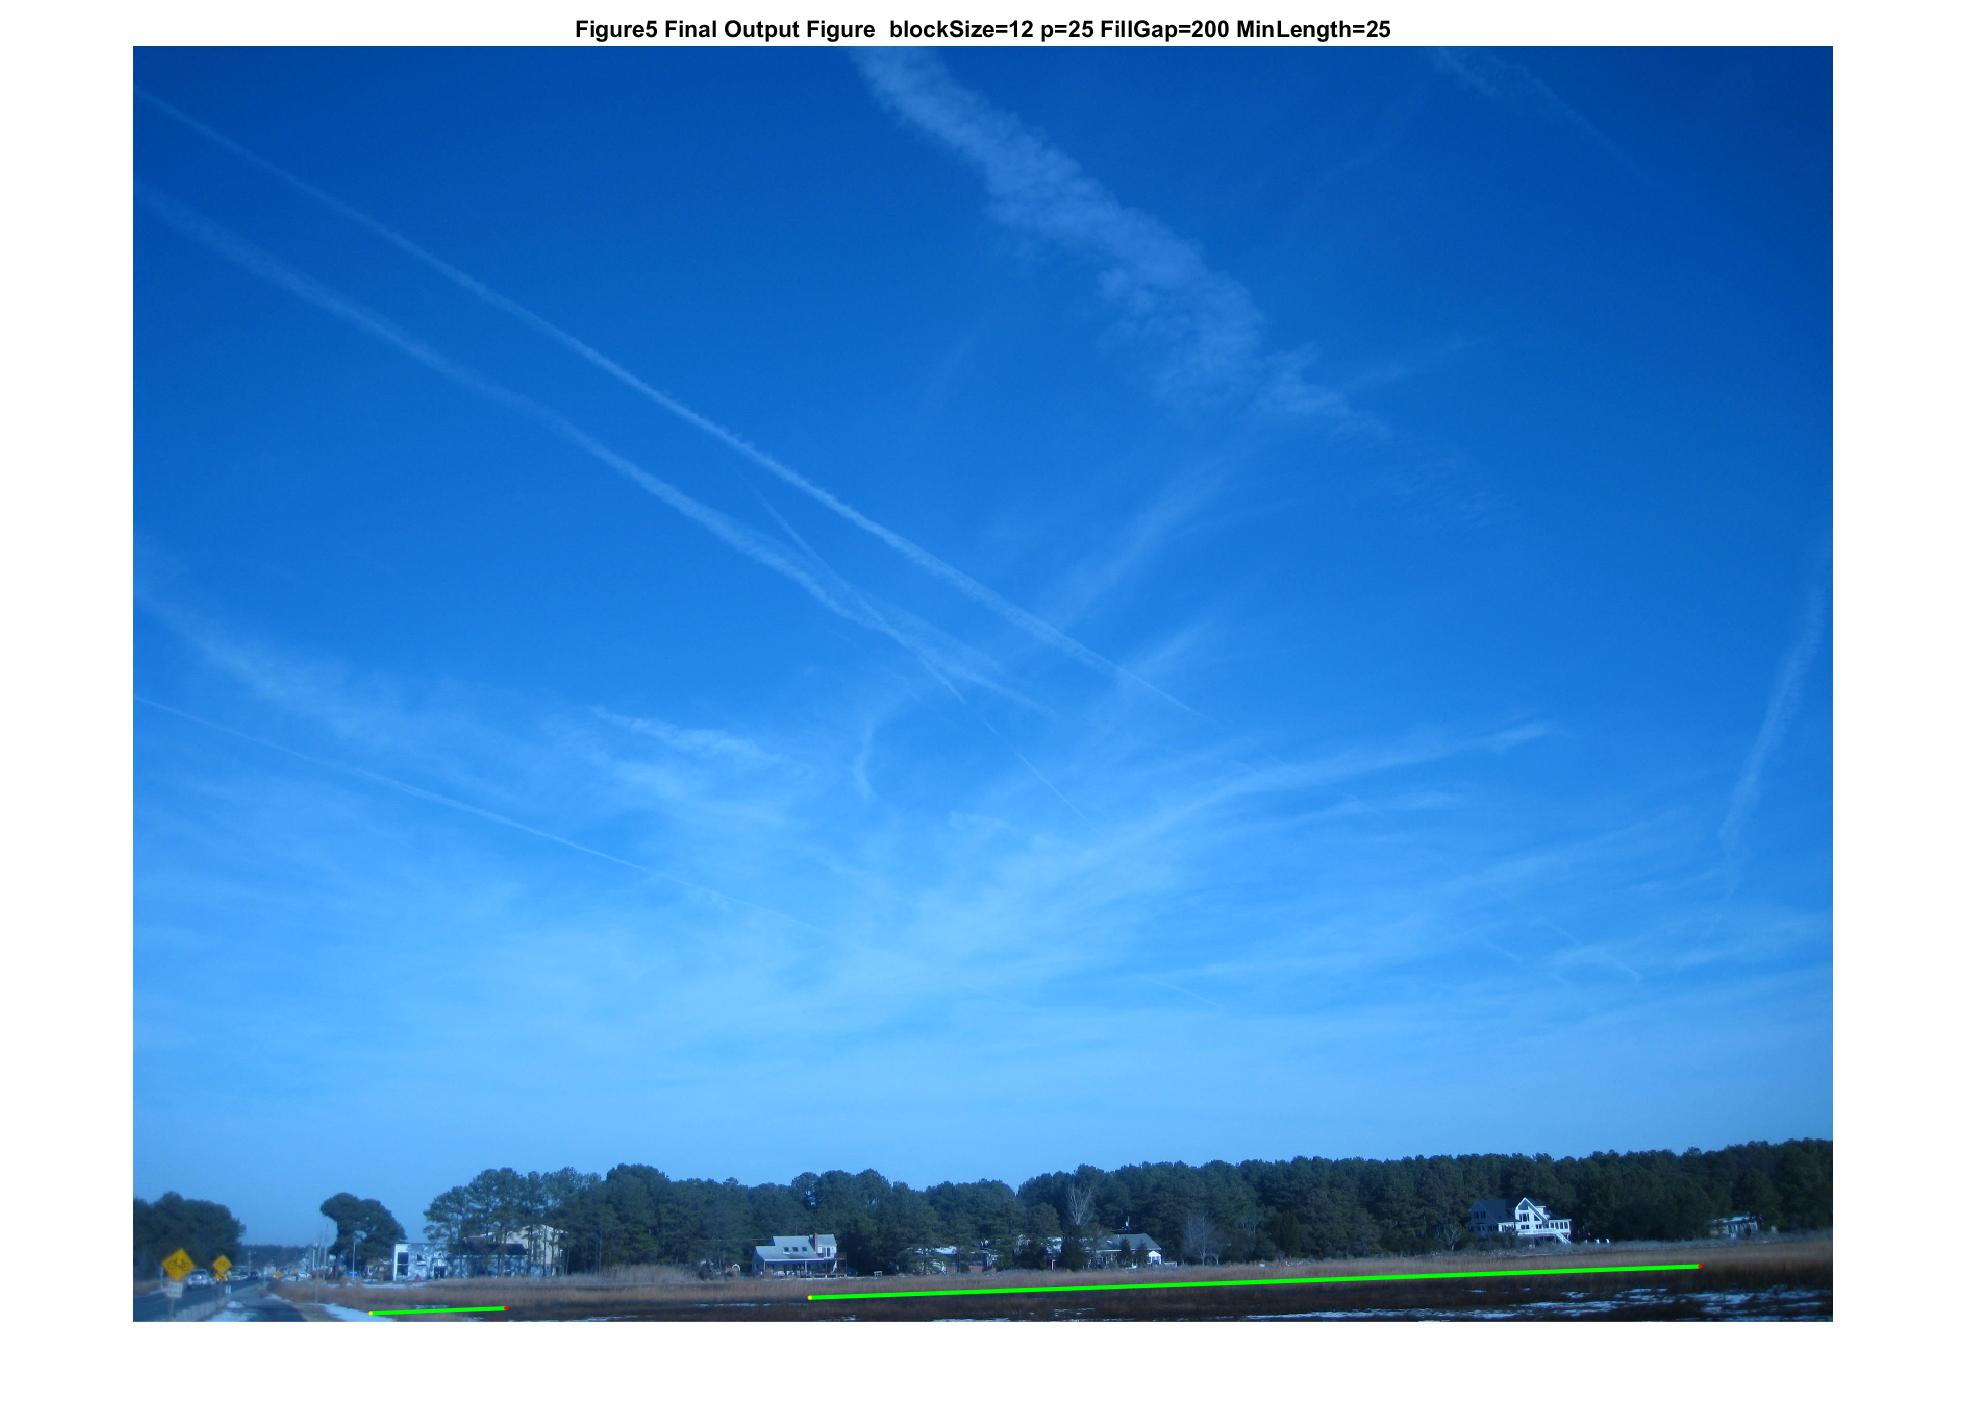
\includegraphics[width=6in]{pic/Figure5_worst.jpg}
	\caption{Worst Result for Figure \ref{figure5}, no contrail covered}
	\label{Figure5_worst}
\end{figure}

\clearpage
\begingroup
\setlength{\LTleft}{-20cm plus -1fill}
\setlength{\LTright}{\LTleft}
{\small
\begin{longtable}{| c | c | c | c | c | c | c | c | c |} \hline
Block & Percentage & FillGap & Minimum & Correct & Incorrect & Missingr & Correct & Incorrect \\
Radius &  & & Length & Number & Number & Number & Rate & Rate \\ \hline
12&15&200&100&3&4&1&75.00\%&57.14\%\\
12&15&200&50&3&5&1&75.00\%&62.50\%\\
12&15&200&25&3&6&1&75.00\%&66.67\%\\
12&5&200&50&2&1&2&50.00\%&33.33\%\\
12&5&200&100&2&1&2&50.00\%&33.33\%\\
12&5&200&25&2&2&2&50.00\%&50.00\%\\
12&15&600&25&2&4&2&50.00\%&66.67\%\\
12&15&600&50&2&4&2&50.00\%&66.67\%\\
12&15&600&100&2&4&2&50.00\%&66.67\%\\
12&15&400&50&2&5&2&50.00\%&71.43\%\\
12&15&400&100&2&5&2&50.00\%&71.43\%\\
12&15&400&25&2&5&2&50.00\%&71.43\%\\
7&5&200&25&1&0&3&25.00\%&0.00\%\\
7&5&200&50&1&0&3&25.00\%&0.00\%\\
7&5&200&100&1&0&3&25.00\%&0.00\%\\
7&5&400&25&1&0&3&25.00\%&0.00\%\\
7&5&400&50&1&0&3&25.00\%&0.00\%\\
7&5&400&100&1&0&3&25.00\%&0.00\%\\
7&5&600&25&1&0&3&25.00\%&0.00\%\\
7&5&600&50&1&0&3&25.00\%&0.00\%\\
7&5&600&100&1&0&3&25.00\%&0.00\%\\
12&5&400&25&1&2&3&25.00\%&66.67\%\\
12&5&400&50&1&2&3&25.00\%&66.67\%\\
12&5&400&100&1&2&3&25.00\%&66.67\%\\
12&5&600&25&1&2&3&25.00\%&66.67\%\\
12&5&600&50&1&2&3&25.00\%&66.67\%\\
12&5&600&100&1&2&3&25.00\%&66.67\%\\
2&25&600&25&1&3&3&25.00\%&75.00\%\\
2&25&600&50&1&3&3&25.00\%&75.00\%\\
2&25&600&100&1&3&3&25.00\%&75.00\%\\
7&15&600&25&1&3&3&25.00\%&75.00\%\\
7&15&600&50&1&3&3&25.00\%&75.00\%\\
7&15&600&100&1&3&3&25.00\%&75.00\%\\
2&25&200&25&1&5&3&25.00\%&83.33\%\\
2&25&200&50&1&5&3&25.00\%&83.33\%\\
2&25&200&100&1&5&3&25.00\%&83.33\%\\
2&25&400&25&1&5&3&25.00\%&83.33\%\\
2&25&400&50&1&5&3&25.00\%&83.33\%\\
2&25&400&100&1&5&3&25.00\%&83.33\%\\
7&15&200&100&1&6&3&25.00\%&85.71\%\\
7&15&400&100&1&6&3&25.00\%&85.71\%\\
7&15&400&25&1&7&3&25.00\%&87.50\%\\
7&15&400&50&1&7&3&25.00\%&87.50\%\\
2&15&200&100&1&9&3&25.00\%&90.00\%\\
2&15&400&25&1&9&3&25.00\%&90.00\%\\
2&15&400&50&1&9&3&25.00\%&90.00\%\\
2&15&400&100&1&9&3&25.00\%&90.00\%\\
2&15&600&25&1&9&3&25.00\%&90.00\%\\
2&15&600&50&1&9&3&25.00\%&90.00\%\\
2&15&600&100&1&9&3&25.00\%&90.00\%\\
2&15&200&25&1&9&3&25.00\%&90.00\%\\
7&15&200&25&1&9&3&25.00\%&90.00\%\\
7&15&200&50&1&9&3&25.00\%&90.00\%\\
2&15&200&50&1&9&3&25.00\%&90.00\%\\
7&25&200&25&1&10&3&25.00\%&90.91\%\\
7&25&200&50&1&10&3&25.00\%&90.91\%\\
7&25&200&100&1&10&3&25.00\%&90.91\%\\
7&25&400&25&1&10&3&25.00\%&90.91\%\\
7&25&400&50&1&10&3&25.00\%&90.91\%\\
7&25&400&100&1&10&3&25.00\%&90.91\%\\
7&25&600&25&1&10&3&25.00\%&90.91\%\\
7&25&600&50&1&10&3&25.00\%&90.91\%\\
7&25&600&100&1&10&3&25.00\%&90.91\%\\
2&5&200&25&0&4&4&0.00\%&100.00\%\\
2&5&200&50&0&2&4&0.00\%&100.00\%\\
2&5&200&100&0&2&4&0.00\%&100.00\%\\
2&5&400&25&0&4&4&0.00\%&100.00\%\\
2&5&400&50&0&4&4&0.00\%&100.00\%\\
2&5&400&100&0&4&4&0.00\%&100.00\%\\
2&5&600&25&0&3&4&0.00\%&100.00\%\\
2&5&600&50&0&3&4&0.00\%&100.00\%\\
2&5&600&100&0&3&4&0.00\%&100.00\%\\
12&25&200&50&0&2&4&0.00\%&100.00\%\\
12&25&200&100&0&2&4&0.00\%&100.00\%\\
12&25&400&25&0&2&4&0.00\%&100.00\%\\
12&25&400&50&0&2&4&0.00\%&100.00\%\\
12&25&400&100&0&2&4&0.00\%&100.00\%\\
12&25&600&25&0&1&4&0.00\%&100.00\%\\
12&25&600&50&0&1&4&0.00\%&100.00\%\\
12&25&600&100&0&1&4&0.00\%&100.00\%\\
12&25&200&25&0&2&4&0.00\%&100.00\%\\ \\\hline
\caption{Experimental results for Figure \ref{figure5}.}
\label{table5}
\end{longtable}
}
\endgroup

\section{Effect of Parameters}
\subsection{Block Radius}
As long as in computer graphics, all the curves are made by the joint of lots of small pieces of line segments. When the block radius is smaller, there must be more blocks can pass the block process to be considered that they are in a straight line. This can make us get more the possible lines. From graph most of the figure results, we can see when the block radius is larger, indeed we can get higher correctness rate. However, if we have more pixels each block pass the algorithm, it means we filter less bad pixels per block, it also increase the incorrectness rate.\\
Also when the block size is larger, the average time to process will be longer.

\subsection{Percentage to Retain}
As I mentioned in 3.3.1, the less percentage will keep less block in the this step.
The block with higher residual value will reminds on the top, thus what we deleted is the blocks less likely to be in the contrails or lines. However, if we have many enough blocks are in lines, a smaller percentage will erase small details of the image which can mislead final result. According to the table, I think 10\% is a good value for this process.

\subsection{Fill Gap}
This parameter will help we find better contrails. Because contrails are not strictly straight lines, there are pixels on contrails may not always lay on the same line. this parameter can help us avoid this kind of problem. Like we discussed for \ref{figure3}, the too small Fill Gap parameter makes the two lines on same contrail were detected as two.\\
However, as long as the Hough Transfer cannot tell if the lines are break because the lines are slightly curved or there is actually lines in between. Thus it will also give us some bad concatenation results. \\
FillGap should be set as property value to make sure it is not either too large or too small when compare with the image size.


\subsection{Minimum Length}
As mentioned in the FillGap, the curves are all made up by small line segments. This parameter is a so important one to make us do not need to see infinitely many line segments. But also, this should keep in a relative threshold of the image to make sure it is in property.


\section{Problems}
This project solution still has some problems:
\begin{enumerate}
\item Parameters need to be manually set if the best result is to be obtained, such as the canny edge threshold; the block size; the r value threshold; and Hough Transform minimum length, minimum gap, line numbers. Otherwise, the results would surprise some details when processing the multiple contrails images.
\item The images with multiple contrails that cross each other will be not be processed well because some blocks which have multiple contrails image cross each other might be deleted because of too large r value.
\item Super large image will be processed very slow because of the pixel by pixel processing algorithm. For example, figure4’s size is 2768 x 1845, and it took 1902 seconds (31.7 minutes) to process it (details see this project package /rst/figure4.txt).
\end{enumerate}
